\documentclass[conference]{IEEEtran}
\IEEEoverridecommandlockouts
% The preceding line is only needed to identify funding in the first footnote. If that is unneeded, please comment it out.
\usepackage{cite}
\usepackage{amsmath,amssymb,amsfonts}
\usepackage{algorithmic}
\usepackage{graphicx}
\usepackage{textcomp}
\usepackage{xcolor}
\usepackage{comment}
\usepackage{booktabs}
\usepackage{url}
\def\BibTeX{{\rm B\kern-.05em{\sc i\kern-.025em b}\kern-.08em
T\kern-.1667em\lower.7ex\hbox{E}\kern-.125emX}}


\begin{document}
    \title{GLOW: Accelerating Geometric Multigrid Levels on Cerebras Wafer-Scale Engine}
    \author{Anonymous Submission}
    \maketitle
    \begin{abstract}
        This paper describes the mapping of Geometric Multigrid (GMG) onto the Cerebras Wafer Scale Engine (WSE-3).  The WSE wafer integrates almost a million cores along with a low-latency 2D mesh network, providing unprecedented on-chip bandwidth and fine-grained communication. Although the architecture is predominantly used for deep learning, we explore the suitability of WSE for accelerating GMG.
        GMG solves sparse linear systems efficiently by recursively coarsening the grid, which leads to more rapid convergence with less computation.
        As compared to prior implementations of stencils on WSE, this demonstration highlights the challenges of mapping a layered algorithm -- and the full set of operators -- onto a dataflow architecture.  We use this implementation as a foundation to discuss the potential for a variety of data and computation mappings of GMG to WSE, and performance compared to the HPGMG benchmark on an NVIDIA H200 GPU.  Across different GMG configurations and problem sizes, we observe a speedup of up to 25\(\times\) as compared to a single H200 node.
    \end{abstract}
    \begin{IEEEkeywords}
        Spatial dataflow architecture, Geometric multigrid, Wafer-Scale Engine
    \end{IEEEkeywords}
    \section{Introduction}
        Geometric multigrid (GMG) is an important family of algorithms used by computational scientists to accelerate the convergence of iterative solvers for linear systems of the form \(Ax=b\). It is a multigrid because computation is mapped to a hierarchy of coarser grid levels.  As shown in Figure~\ref{fig 1:V-cycle in GMG}, the underlying GMG operators are organized in a V-cycle that includes stencil application, residual, restriction, interpolation, smooth, and a direct (bottom) solver. In such a formulation, the floating-point computation in GMG is dwarfed by the overhead of data movement (during stencil application and across levels), making managing the memory hierarchy and cross-processor communication critical to achieving high performance. The best-performing algorithm for multigrid solutions has always been driven by the architecture: for decades the focus has been on distributed-memory CPU clusters, and, more recently, by accelerators such as GPUs. While these systems deliver high peak floating-point throughput, the performance of the dominant smooth and bottom solver in multigrid is often memory-bound, limited by cache hierarchies, off-chip DRAM bandwidth, and the cost of communicating across nodes over high-latency interconnects. 
        %These bottlenecks constrain scalability, especially for stencil-based solvers and multigrid methods whose arithmetic intensity is low. 

        \begin{figure}[th]
            \centering
            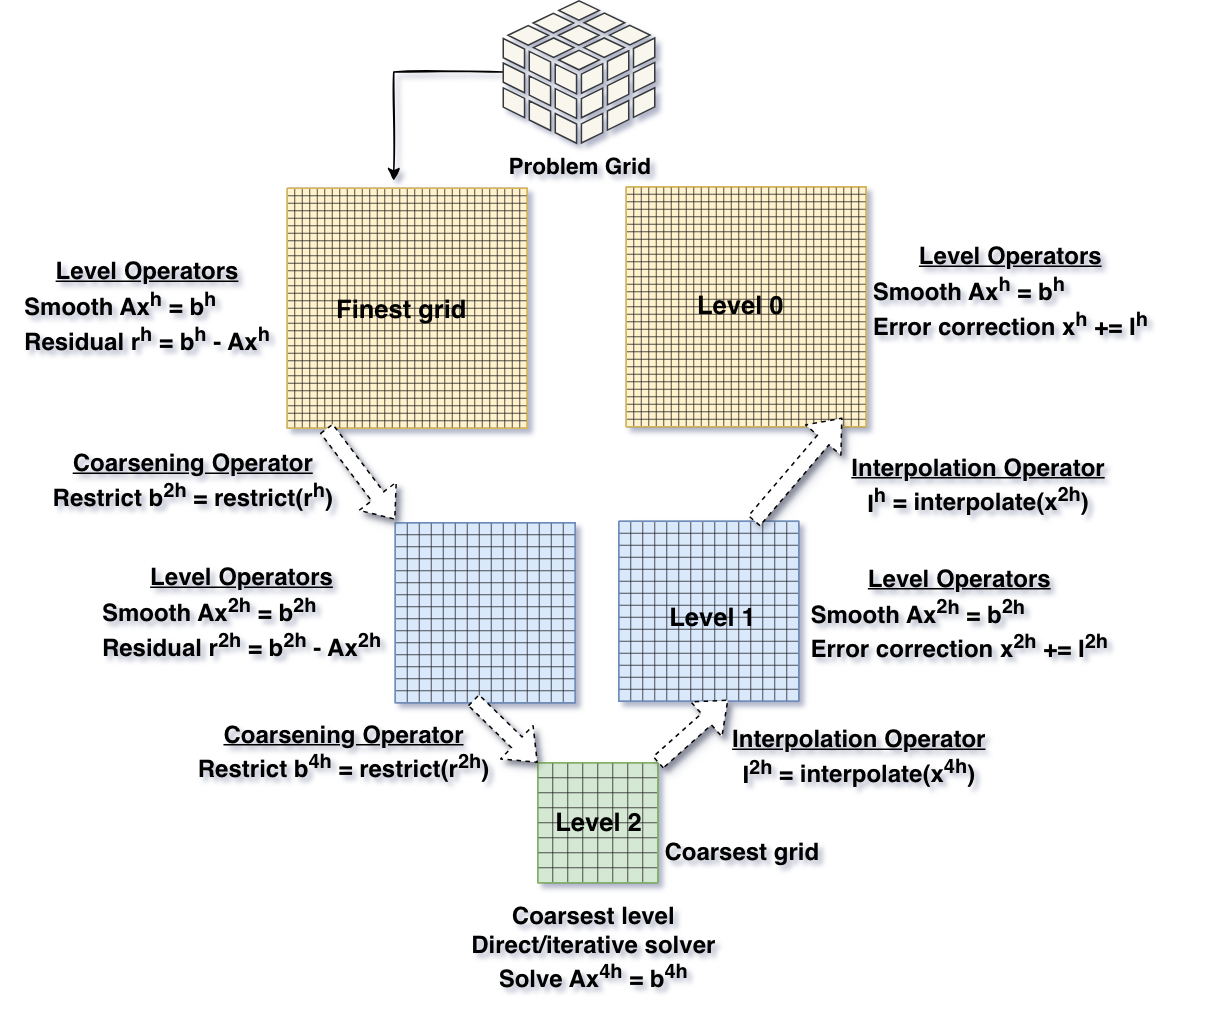
\includegraphics[width=1\linewidth]{figures/fig1_gmg_v_cycle.drawio (2).png}
            \caption{Schematic representation of a Geometric Multigrid V-cycle illustrating smooth, restriction, coarse-grid correction, and interpolation operators. Small 3D grid represents the problem domain}
            \label{fig 1:V-cycle in GMG}
        \end{figure}

        This paper presents and evaluates the implications of mapping GMG to the Cerebras Wafer-Scale Engine (WSE), a radically different architectural model~\cite{Cerebras,Lauterbach}. By integrating nearly one million processing elements (PEs) and tens of gigabytes of on-wafer SRAM onto a single wafer-scale chip, the WSE provides single-cycle access to local memory and 21 petabytes-per-second of memory bandwidth, along with 214 petabits-per-second of fabric bandwidth through a 2D mesh interconnect. 
        As a result, algorithms that are typically memory-bound on CPUs and GPUs frequently become compute-bound when ported to the WSE.  Prior work has demonstrated this shift for diverse workloads such as stencil computations~\cite{Sai,sai2,Rocki,scalable_25pt_stencil,mathias}, seismic analysis~\cite{Ltaief}, molecular dynamics~\cite{perez_md_sc24,perez-journal}, and Monte Carlo particle transport kernels~\cite{Tramm24,Yoshii26}.
        In this paper, we present GLOW (Gmg Levels On Wafer).  We build on the lessons from successful use of Cerebras for stencil computations to provide a mapping of an algorithm that is still structured yet significantly more challenging.
        
        Our paper is centered around an iso-capability (same problem size) study of the WSE (44GB of SRAM) and a GH200 GPU (96 GB of HBM DRAM).  We present a dispassionate performance analysis of the WSE-3 focusing on the relevant benefits and pitfalls associated with massive decoupled thread parallelism, and planar network topologies for multi-scale computations.  As compared to a GH200 GPU implementation of the HPGMG benchmark, we achieve significantly improved performance.  At the same time,
        the implementation of GMG must address new challenges on the Cerebras architecture: (1) limitations on problem size that fit on the wafer; (2) relative communication costs growing at deeper levels of the V-Cycle; and, (3) trading off code size and data space in the memory-constrained tile.
        %This fine-grained distributed-memory architecture eliminates traditional cache hierarchies and drastically reduces memory latency both on PE and across PEs.
        %Despite these successes in stencils, what remains missing is a demonstration of scientific computing workloads that go a step beyond traditional stencil kernels. 
        %, while important, are now a well explored class of applications on this dataflow machine, and several efforts have replicated or extended these patterns but yet to address a more realistic, end-to-end use case. From the perspective of the Berkeley “Seven Dwarfs” [citeme] taxonomy, \textit{structured grids} represent a key category of scientific workloads that to our knowledge have not been explored on this hardware, particularly in the context of large-scale PDE solvers. This gap highlights the need to push beyond simple 7-point or 25-point stencils towards workloads that are 
        %Geometric Multigrid (GMG) serves as a manageable proxy application for real-world PDE solvers, %(Adaptive Mesh Refinement(AMR)), 
        %while introducing algorithmic complexity that stresses the architecture in %nontrivial 
        %several ways. GMG incorporates richer loop structures, multi-level communication, data movement patterns across PEs and in particular different layer mapping strategies, in its smoother, restriction, and interpolation phases. Geometric Multigrid (GMG) exploits the structured hierarchy of the underlying mesh and operates in a matrix-free fashion, relying on stencil computations rather than storing the full sparse matrix, a property that is both memory-efficient(48KB memory) and compute-friendly [cite: PDE \& discretization slides; Sam slides]. 
        %\textcolor{red}{The implementation details (like CSL) are too low-level for the intro.  I don't think you should say things like hop-based and window-based either, especially since they are not defined.  This paragraph could summarize the findings, for example: \textit{

        %These results suggest several adaptations of the multigrid algorithm to maintain the benefits of low memory latency within the tile and fast nearest neighbor communication.  %such as ??? shallower levels and more like a W-cycle, lower-order of stencil due to less memory, ...???
        %In this work, we accelerate the Geometric Multigrid Layers using a distributed-dataflow mapping strategy onto the WSE-3. We have implemented a Geometric Multigrid algorithm using CSL, a low level Zig-based kernel programming language for writing dataflow programs on Cerebras.  Our implementation relies on a hop-based 7-point stencil implementation and a window based reduction pattern. 

        This paper makes the following contributions:
        \begin{itemize}
            \item The first implementation of a multigrid algorithm on Cerebras WS-3, to the best of our knowledge.
            \item A performance model of communication costs, along with a forwarding communication optimization, using the strided distributed solution we propose.
            \item Extensive performance measurements, including per-operator and per-level cost, along with a comparison with an NVIDIA GH200 running HPGMG that exhibits speedup of up to \(25\times\).
            \item Lessons regarding GMG algorithm configuration suitable for a tiled architecture with limited memory.
        \end{itemize}

    \section{Background}
        This section summarizes the GMG approach and the key aspects of the Cerebras architecture relevant to this study.

        \subsection{Geometric Multigrid Methods}

            Multigrid methods are iterative solvers which solve sparse linear system of equations by forming a hierarchy of grid levels and iterating across them to %eliminate errors efficiently. 
            improve accuracy.  %The key idea is to convert the high-frequency errors from finer grids into low-frequency errors and solve them at the coarsest grid. 
            Geometric Multigrid (GMG) specifically uses the geometry of the problem to construct different levels and the grid hierarchy, as illustrated in Figure~\ref{fig 1:V-cycle in GMG}.
            %The finest level contains the largest amount of data and computation, and each successive level typically halves the grid resolution. A GMG cycle begins with an initial approximation on the finest grid and recursively improves it across the hierarchy to generate correct solution.
            In the figure,
            %Fig \ref{fig 1:V-cycle in GMG} illustrates 
            a three-level V-cycle is used to solve (\(Ax = b\)), where (A) is the stencil operator, (x) is the solution, (b) is the right-hand side, and superscripts (h), (2h), and (4h) correspond to grid spacings. Each level performs two primary operations: smoothing and residual evaluation. The smoother reduces high-frequency error, commonly with % by approximately solving the equation (\(A^h x^h = b^h\)), commonly used method is 
            the weighted Jacobi smoother. %, expressed as \[x_1^h = x + w(b^h - A^hx)\]
            %where w is the weighted Jacobi coefficient and \(x_1^h\) explicitly shows the new smoothened value of \(x\). 
            The residual operator %computes \[r^h = b^h - A^h x^h\] which 
            measures the deviation of the current iterate from the exact solution. The coarsening step restricts the residual to the next level, generating the coarse-grid right-hand side. %\[b_2h  = Restrict(r^h)\]

            In finite-volume discretizations, restriction corresponds to averaging the contributions of eight fine-grid cells into one coarse cell, recursively repeated %The algorithm continues this process 
            until reaching the coarsest grid, where the system is sufficiently small to be solved with a direct or iterative method such as conjugate gradient, BiCGSTAB or Jacobi. %Common bottom solvers include Conjugate Gradient (CG), Preconditioned CG (PCG), and BiCGSTAB or even a Jacobi smoother. 
            After the coarse solution is computed, the V-cycle traverses back up through the hierarchy. Interpolation transfers the coarse-grid correction to the finer grid %using  \[I^2h = Interpolate(x^4h)    >> TODO: Fixme\] Where in interpolate 
            such that a single coarse cell is replicated to 8 fine cells, the inverse of restriction. An error-correction step updates the fine-grid solution. % using  \[x^2h = x^2h + I^2h        >>  TODO: Fix me\]
            Finally post smoothing reduces any high-frequency errors reintroduced during interpolation. This down-and-up traversal is called a V-cycle, and achieves rapid convergence.
            %technique produces rapid convergence, alternative cycles, include W-cycles and F-cycles.
            %The most expensive computation in GMG is the sparse matrix–vector (SpMV) multiply that appears in smoothing and residual. In structured-grid problems, this operation is implemented in a matrix-free form using stencil operators one such 3D-7 point Laplacian operator. No explicit matrix is stored, which reduces memory and improves locality. The total time of a multigrid is the number of iterations multiplied by the time for one V-cycle shown in equation (1). 
            The cost of each V-cycle depends on the number of levels, the choice of operators and coarse-grid solver, the number of iterations on the coarse solver, and the performance of the stencil computation. Optimizing GMG therefore requires reducing the time spent in each operator %, specifically Stencil operator 
            and the interactions between levels. %\textcolor{red}{OA: rewrite the last sentence, "optimizing" is everywhere}
            %\[TimeTotal = iterations * TimePerV-cycle\]
            %\textcolor{red}{You need to list all of the operators and their goals}
            %\textcolor{red}{The V-cycle should have been at the beginning of this section.  This is late.}
            %\textcolor{green}{Todo: Seems like some pieces can be trimmed, dumped as of now}

            \begin{figure}[ht]
                \centering
                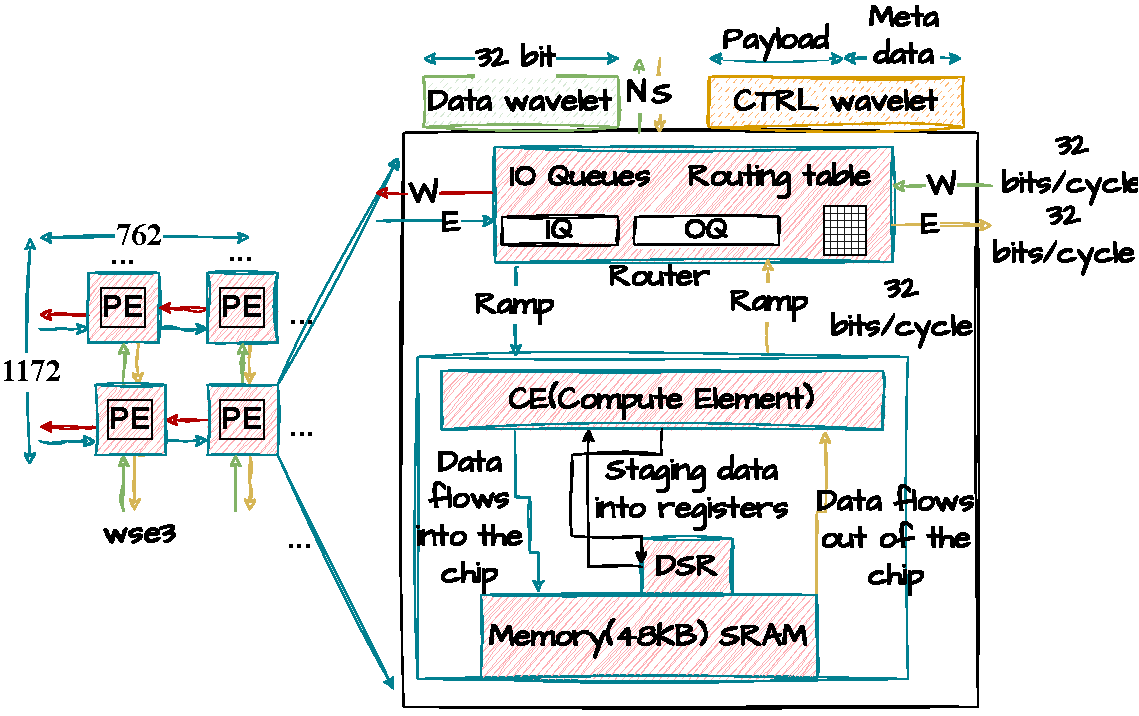
\includegraphics[width=1\linewidth]{figures/WSE2_v2.pdf}
                \caption{A schematic representation of WSE-3, %. The WSE is 
                a 2D grid structure where %made up of dies and 
                each die is made of processing elements (figure left). %Figure shows a virtual concept of colors used to design routing paths, 
                Figure right shows the hardware machinery inside a PE: router, memory and  Compute Element (CE). The WSE-3 system is a giant 46,255 mm² chip along with the machinery needed to cool, power and provide I/O.} %\textcolor{blue}{Increased font please check if readable}}
                \label{fig:CS3}
            \end{figure}

        \subsection{Cerebras WSE-3 and Programming Model}
            Figure~\ref{fig:CS3} shows the schematic representation of Cerebras WSE-3 Wafer-Scale Engine.
            The wafer  consists of  893{,}064 identical, simple Processing Elements (PEs) arranged in a homogeneous 1172\(\times\)762 2-dimensional grid. Each PE is self-contained with its own Memory, Compute Element (CE) and Router; i.e.,  the WSE is a spatial, distributed-memory, and dataflow-oriented architecture. %PEs don't share data unless communicated explicitly through the fabric. 

            \subsubsection{Router}
                A 5-port router moves the data across neighboring PEs (East, West, North, South links) and the CE (Ramp link) using 32-bit \textit{wavelets}, the fundamental unit of communication. Routing is defined by 24 static virtual channels, called \textit{colors}.  In Figure~\ref{fig:CS3}, the colors red, blue, green and yellow show the routing of data into and out of the chip from neighboring directions (N,S,E, and W). %along with types of wavelets over a color channel.
                A wavelet is assigned to a color, which encodes a routing path across PEs. A router decides, based on the wavelet's color and its configuration, where to send the wavelet.
                %of the wavelet and the configuration of router where should the wavelet go next.  
                Multicasting replicates the wavelet and sends it in all directions with zero cost overhead. The router also has Queues for input output buffering.

                For dynamic routing, the system provides \textit{control wavelets}, which include additional metadata that allows routers to update entries in their routing tables at runtime and to trigger control tasks. %This enables runtime reconfiguration when static colors are exhausted or algorithmic phases require different communication patterns. The router maintains input and output queues, and supports multicast by replicating wavelets in multiple directions at essentially no additional cost.  
                All links operate at 32 bits per cycle.
                %\textcolor{red}{I commented out multicast and input/output queues.  We can add back if used later in the paper.}
                %\textcolor{blue}{We are using in the optimization, we can add it back now. }

            \subsubsection{CE and Memory}
                The CE executes integer and floating-point operations and includes FP16 and FP32 SIMD instructions
                %-like tensor traversal mechanisms[citeme?] 
                that enable fast access to local memory. The CE consists of one main thread and up to eight microthreads, each of which may perform computation or handle I/O wavelets; in this way, computation and communication are overlapped.
                %which allow computation to overlap with communication allowing each microthread to handle I/O wavelets and thread to perform computation. FP16 and FP32 operations can be issued through wide SIMD execution units, and a
                A small set of Data Structure Registers (DSRs) provide lightweight staging of data to/from the local 48KB SRAM, as shown in the figure. %Given no cache hierarchy, performance comes from the data movement of local 48KB SRAM access, and using tensor access patterns to read and write memory efficiently and using SIMD registers shown as Data Structure Registers(DSR) in the figure to stage the data. 
                No data cache is needed since memory accesses exhibit %The memory is 
                single-cycle latency with 64-bit writes/cycle and 128-bit reads/cycle~\cite{luczynski_reduce}.
                %\textcolor{red}{check CS3?}. 
                In total, the wafer has 44 GBytes of on-chip SRAM memory.  %fast SRAM memory on chip.

                %\textcolor{red}{This subsection has good content, but should be shorter.  You should focus on things relevant to the paper content.}

            \subsubsection{Programming Model}
                \label{sec:programmingmodel}
                %Unlike CPU or GPU programming, which abstract away memory hierarchies or thread scheduling, CSL requires developers to explicitly define both computation and communication. 
                The programming interface, known as the Cerebras Software Language (CSL), exposes typical constructs including loops, functions, and conditionals, as well as low-level constructs such as Data DSDs, %\textcolor{red}{OA: fix the parentheses or avoid them }, 
                colors for routing, asynchronous tasks, and runtime router configuration~\cite{CSL}. Typically, %like host-accelerator programming models, 
                the host code is written in Python where the programmer manages the initial data copy onto the spatial tiles along with allocation of tensors. %The kernels written in 
                CSL kernels manage the allocation of data on each PE and the corresponding computations. CSL layout code defines colors and routing across PEs; it also maps the kernel code spatially across the million PEs.

                A CSL kernel consists of \textit{functions} and \textit{tasks}; data and control tasks describe dataflow, and execute only after being activated. %where tasks are the mechanism to enable dataflow. There are 3 types of tasks: data task, control task and local tasks, these cannot be invoked like function instead can be activated. These Wavelet-triggered tasks(data and control) are activated 
                Activation occurs when a wavelet tagged with a particular virtual channel (color) arrives at the PE’s router, which can further trigger a change in router configurations or perform computations on the data. %, enabling a pure dataflow programming experience. On the other hand l
                There are also local tasks that must be explicitly activated. %\textcolor{red}{OA: same here, there is no need of the () or use it before the punctuation}
                This wavelet-triggered task model offers %high level of 
                asynchronous fine-grained parallelism, but requires the programmer to manage communication and synchronization. %although the programmer has to be careful about managing synchronization across these tasks and not get stuck with deadlocks. To overcome such challenges a task can be blocked or unblocked to explicitly gain control over it's execution. 

                %\textbf{Motivating para and connect to GMG/MG:}
                %\subsubsection{Example}
                %    Together these features establish an asynchronous fine-grained distributed dataflow model where wavelets serve as messages and colors define communication channels, effectively treating a million distributed PEs as a coherent, programmable network. %\textcolor{green}{By abstracting away the complexity of conventional MPI-style distributed computing}, this paradigm allows developers to program the entire fabric as a single chip while exploiting massive parallelism. However, it demands a careful design and fundamental rethink of data placement, routing and locality; particularly for multilevel algorithms like GMG, where varying computation and communication patterns make spatial layouts and mapping strategies critical to performance.
                %Furthermore, collective operations such as row-wise reductions, broadcasts, timers are available as built-in primitives, but developers can also design custom routing patterns in layout files to tailor communication for their specific algorithms. 
                %\textcolor{red}{I commented out most of the paragraph that is supposed to connect to GMG, as it does not currently do that.  But I like the suggestion below of a small code example so I left the first sentence.  It could also be deleted.}
                % %\textcolor{green}{TODO: I have idea of a figure with 3 boxes, python, kernel csl, layout csl side by side a small minimal code example?}

                \begin{figure}[t]
                    \centering
                    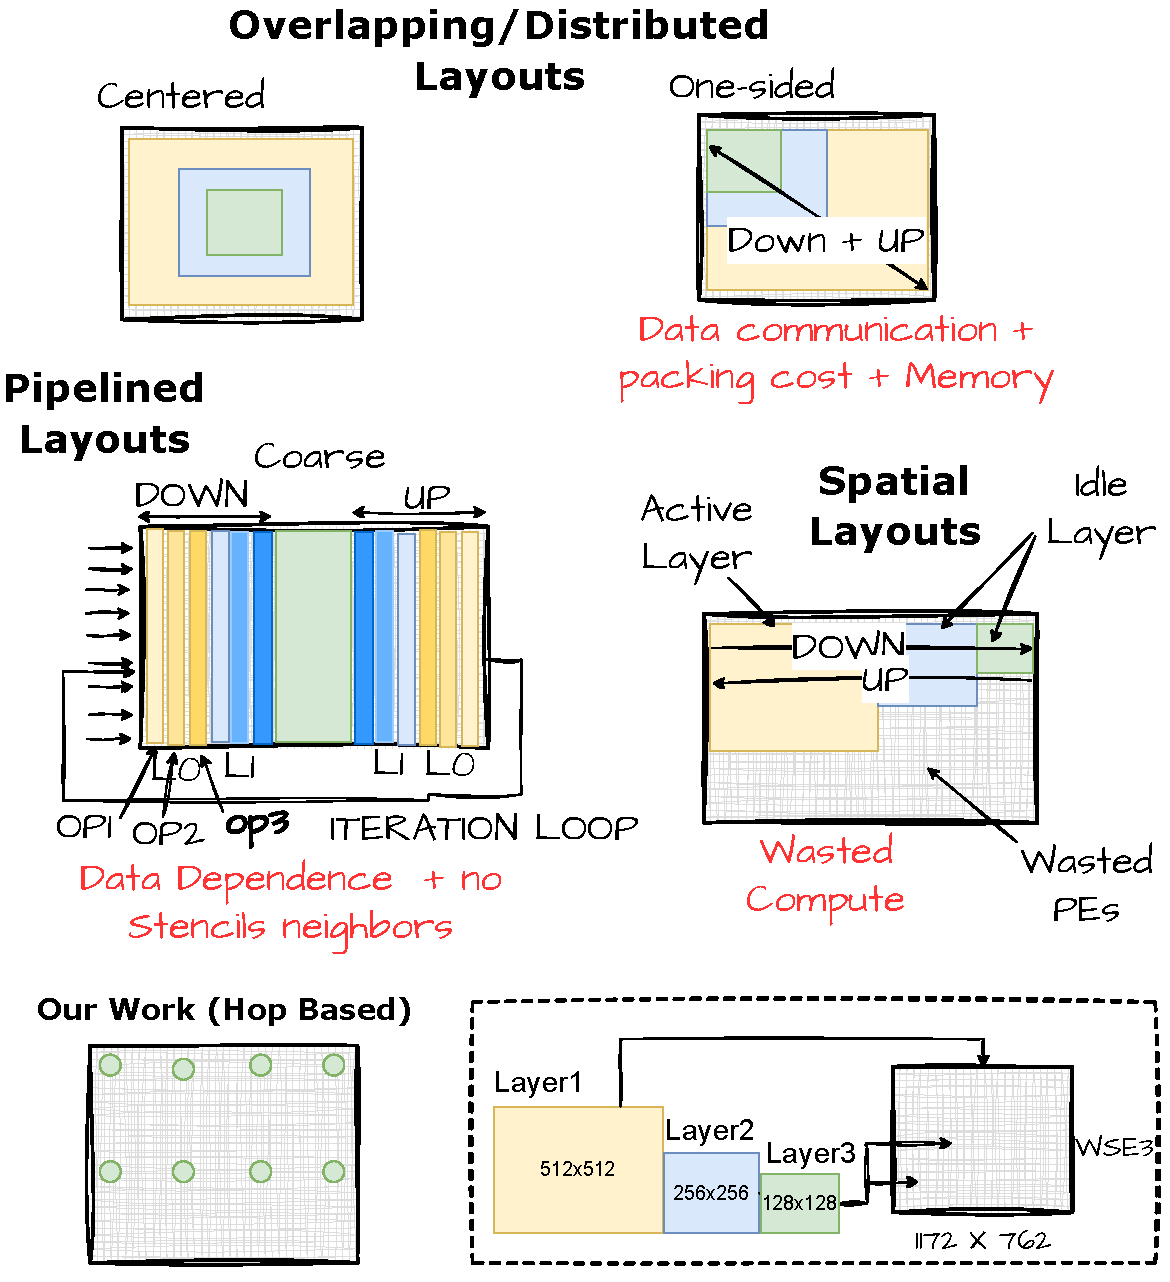
\includegraphics[width=0.9\linewidth]{figures/layouts_vertical.pdf}
                    \caption{Different possible layouts for 3 level GMG layers on WSE3 of size 1172x762. Text in red highlights various challenges of each approach. Our approach falls into the distributed category. }
                    \label{fig:VariousLayouts}
                \end{figure}

                \begin{figure}[t]
                    \centering
                    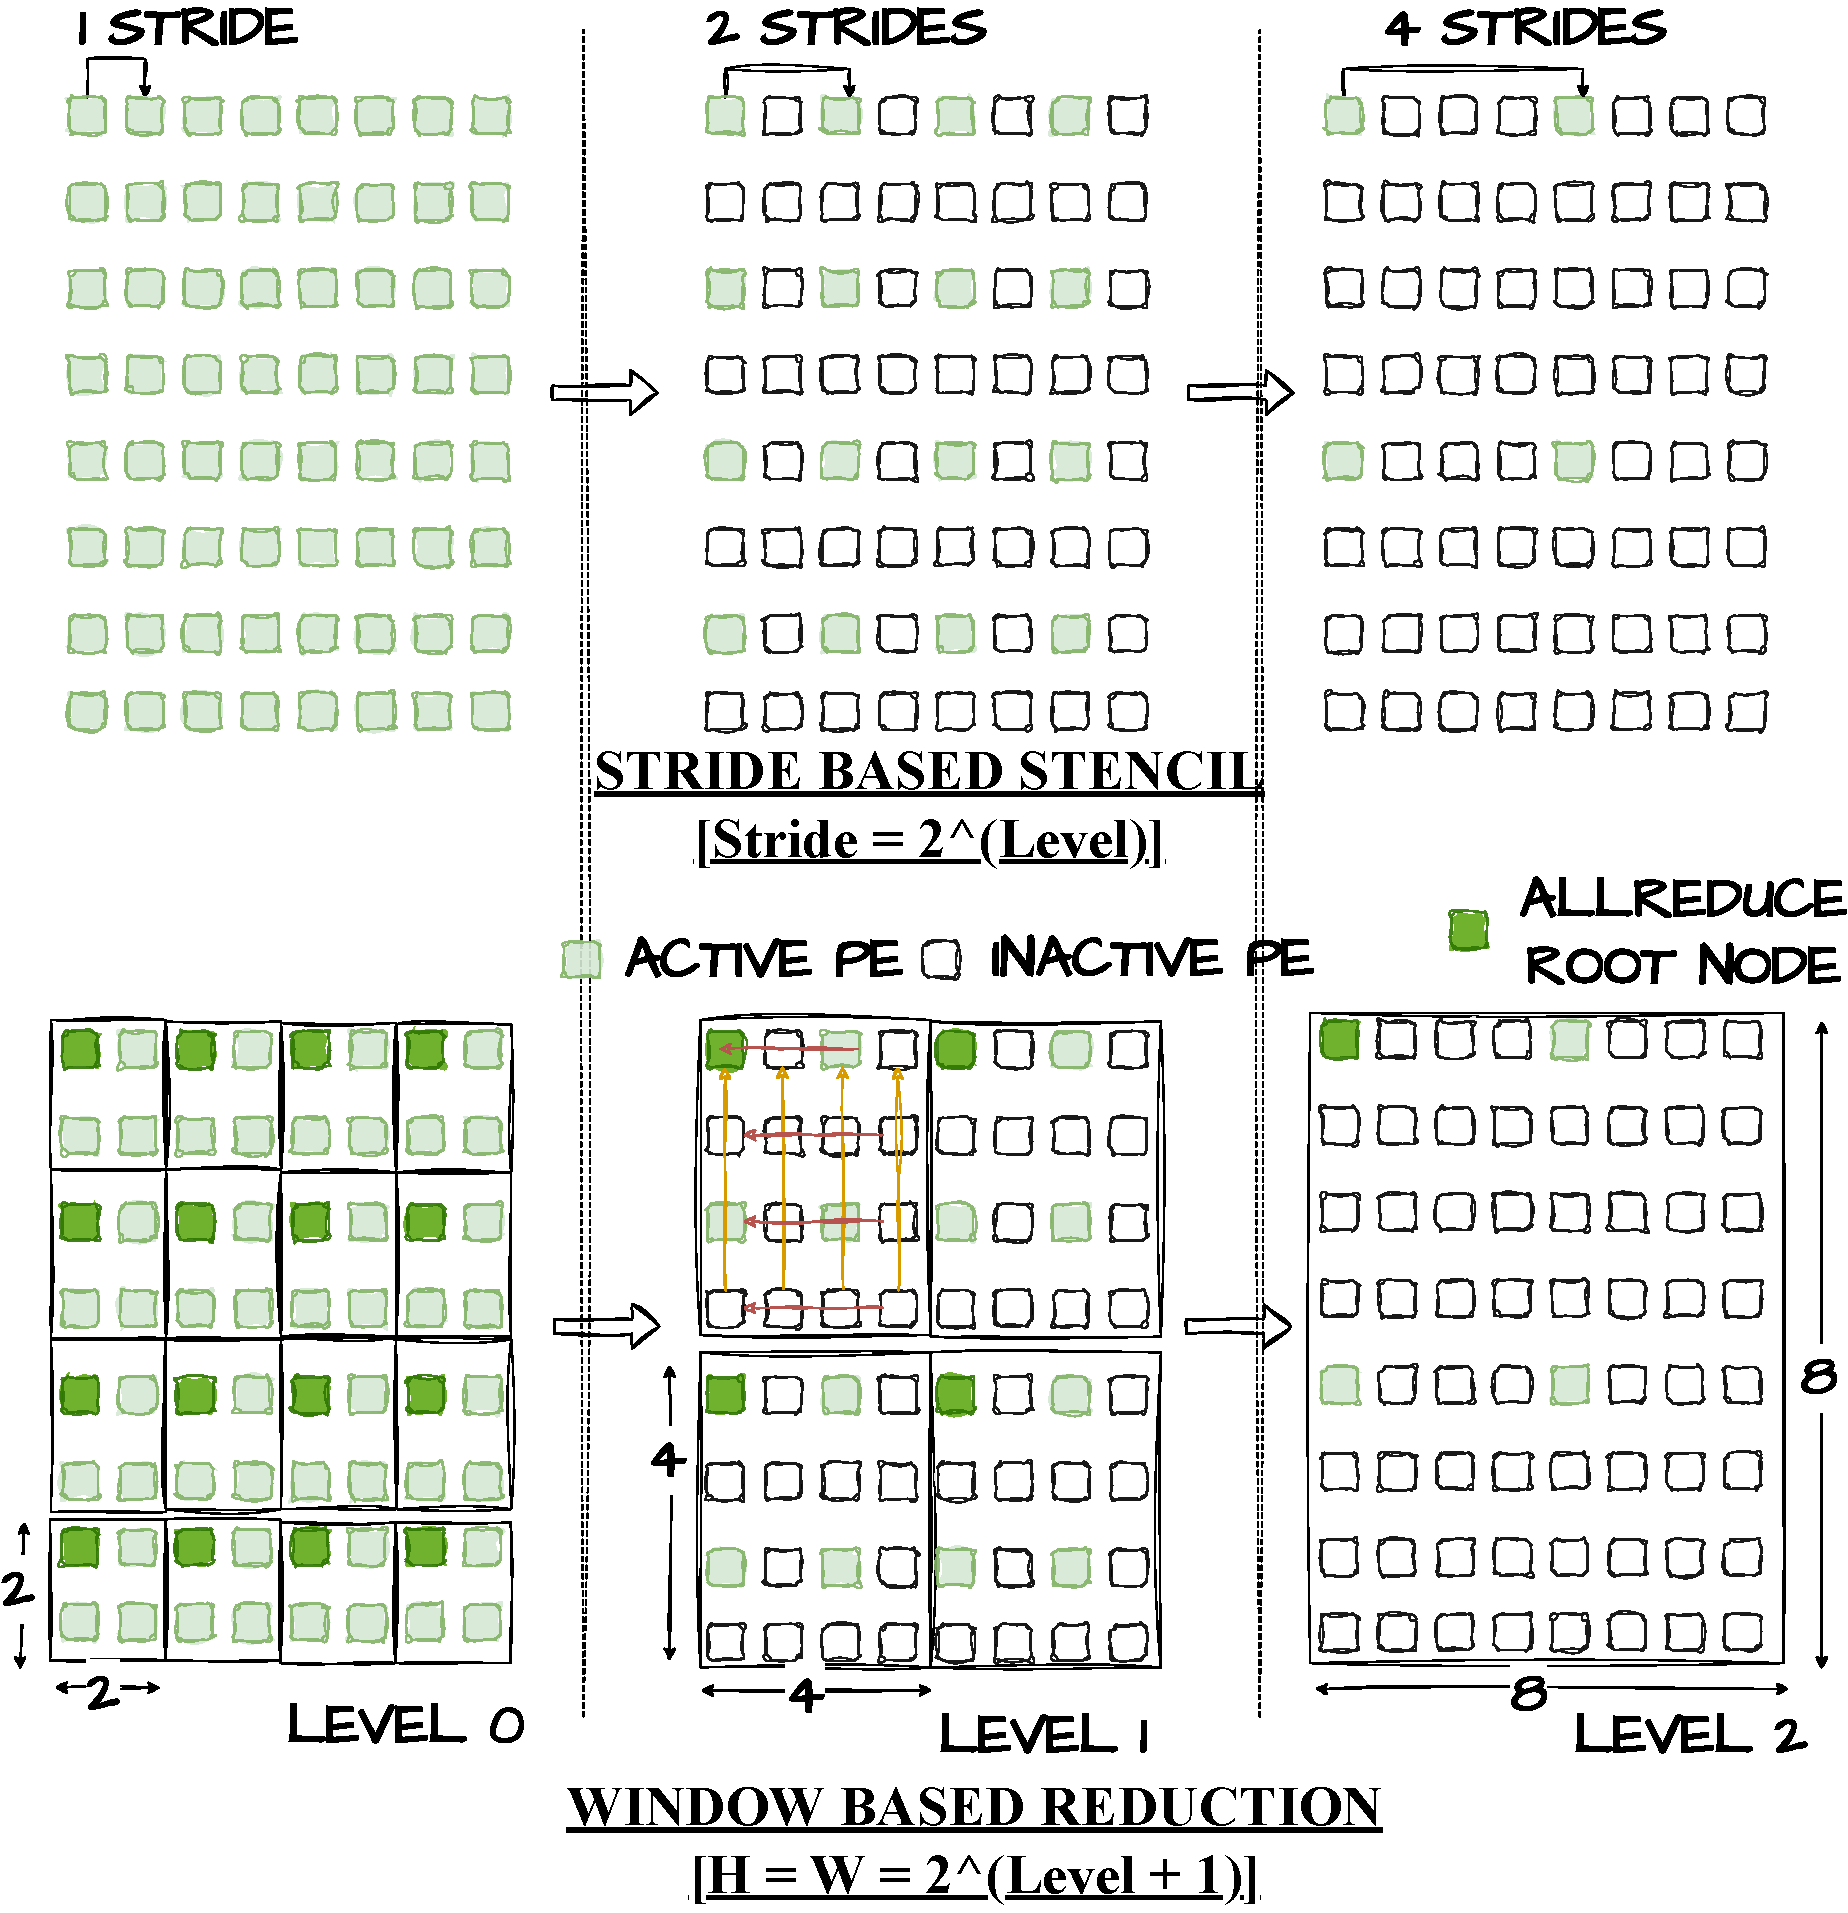
\includegraphics[width=0.95\linewidth]{figures/spmp_restriction.pdf}
                    \caption{Top: Stencil Operator on WSE-3 2D grid for a \(8^3\) problem with 3 levels. The Highlighted nodes are the Active PEs and remaining Inactive PEs. The Hop distance differs as one keeps going down the levels and the SpMV exchanges halo regions H hops apart }
                    \label{fig:Spmv_and_restriction}
                \end{figure}

\begin{comment}
                    \begin{table*}[t]
                    \centering
                    \caption{Comparison of layout strategies for mapping GMG to WSE-3. Utilization refers to the amount of chip used. Green indicates low overhead, Orange moderate overhead, and Red high overhead.}
                    \label{tab:layout_comparison}
                    \renewcommand{\arraystretch}{1}
                    \setlength{\tabcolsep}{3pt}

                    % \begin{tabular}{@{}lccccccc@{}}
                    %     \toprule
                    %     \textbf{Strategy} 
                    %     & \begin{tabular}[c]{@{}c@{}}\textbf{Memory-Usage}\\\textbf{/PE}\end{tabular} 
                    %     & \begin{tabular}[c]{@{}c@{}}\textbf{Routing-Color}\\\textbf{Complexity}\end{tabular} 
                    %     %& \begin{tabular}[c]{@{}c@{}}\textbf{Stencil}\\\textbf{Library}\\\textbf{Compatible}\end{tabular} 
                    %     & \begin{tabular}[c]{@{}c@{}}\textbf{Halo-Exchange}\\\textbf{Locality}\end{tabular}  
                    %     & \begin{tabular}[c]{@{}c@{}}\textbf{Inter-level/}\\\textbf{Cost}\end{tabular}  
                    %     & \begin{tabular}[c]{@{}c@{}}\textbf{Intra-level/}\\\textbf{Repacking}\\\textbf{Cost}\end{tabular}  
                    %     & \textbf{Utilization} 
                    %     & \begin{tabular}[c]{@{}c@{}}\textbf{Coarse-level}\\\textbf{sensitivity}\end{tabular} \\
                    %     \midrule
                    %     Spatial      & {\color{green} Low} & Low      & High  & Low   & High   & Low         & Low      \\
                    %     Pipeline     & Low   & Low      & High  & Low   & High   & High         & Medium      \\
                    %     One-side overlapped   & High   & High    & High  & Low   & High   & Medium         & Low      \\
                    %     Centered-overlapped & High   & High     & High  & Low   & Medium   & Medium       & Low      \\
                    %     Strided (this paper) & High   & High    & Varies  & High   & Varies   & High         & High      \\
                    %     \bottomrule
                    % \end{tabular}


                    \begin{tabular}{@{}lccccccc@{}}
                    \toprule
                    \textbf{Strategy}
                    & \begin{tabular}[c]{@{}c@{}}\textbf{Memory-Usage}\\\textbf{/PE}\end{tabular}
                    & \begin{tabular}[c]{@{}c@{}}\textbf{Routing-Color}\\\textbf{Complexity}\end{tabular}
                    & \begin{tabular}[c]{@{}c@{}}\textbf{Halo-Exchange}\\\textbf{Locality}\end{tabular}
                    & \begin{tabular}[c]{@{}c@{}}\textbf{Inter-level}\\\textbf{Cost}\end{tabular}
                    & \begin{tabular}[c]{@{}c@{}}\textbf{Intra-level}\\\textbf{Repacking}\\\textbf{Cost}\end{tabular}
                    & \textbf{Utilization}
                    & \begin{tabular}[c]{@{}c@{}}\textbf{Coarse-level}\\\textbf{sensitivity}\end{tabular}             \\
                    \midrule
                    Spatial
                    & {\color{green} Low}
                    & {\color{green} Low}
                    & {\color{green} High}
                    & {\color{green} Low}
                    & {\color{red} High}
                    & {\color{red} Low}
                    & {\color{green} Low}                                                                             \\

                    Pipeline
                    & {\color{green} Low}
                    & {\color{green} Low}
                    & {\color{green} High}
                    & {\color{green} Low}
                    & {\color{red} High}
                    & {\color{green} High}
                    & {\color{orange} Medium}                                                                         \\

                    One-side overlapped
                    & {\color{red} High}
                    & {\color{red} High}
                    & {\color{green} High}
                    & {\color{green} Low}
                    & {\color{red} High}
                    & {\color{orange} Medium}
                    & {\color{green} Low}                                                                             \\

                    Centered-overlapped
                    & {\color{red} High}
                    & {\color{red} High}
                    & {\color{green} High}
                    & {\color{green} Low}
                    & {\color{orange} Medium}
                    & {\color{orange} Medium}
                    & {\color{green} Low}                                                                             \\

                    Strided (this paper)
                    & {\color{red} High}
                    & {\color{red} High}
                    & {\color{orange} Varies}
                    & {\color{red} High}
                    & {\color{orange} Varies}
                    & {\color{green} High}
                    & {\color{red} High}                                                                              \\
                    \bottomrule
                    \end{tabular}
                    \vspace{1mm}

                    %\textit{Notes:} 
                    %``Memory footprint'' considers per-PE storage; ``Routing \& coloring complexity'' reflects implementation effort and configuration overhead; ``Stencil locality'' refers to the spatial proximity of stencil neighbors supporting efficient communication; ``Inter-level'' and ``intra-level'' cost capture data movement between/coarse levels and within a single level, respectively; ``\#Idle PEs'' encodes potential underutilization; ``Coarse-level sensitivity'' relates to mapping efficiency as levels become coarser; ``Repacking cost'' highlights the memory and communication required to move or densify the grid for operator application.
                    %\textcolor{red}{NOT SURE THIS IS NECESSARY, BUT MARKING I: Note: We are talking about stencils by default in all mapping.  We are also talking about iterations, which adds cost.[TODO:fill]}
                    \end{table*}
\end{comment}


    \section{Mapping GMG to WSE-3}
        This section describes our mapping of GMG onto the WSE-3 wafer.  We first consider the pros and cons of alternative approaches for mapping the problem grid and multi-grid levels onto the PEs in Section~\ref{sec:mapping_alternatives}.
        We describe the layout of the multi-grid data in Section~\ref{sec:data_layout}. %We describe the implementations of the operators, and discuss optimization opportunities.  
        Task activation is managed with a State Machine, as described in Section~\ref{sec:statemachine}.  The design of key operators and a model of their communication are presented in Section~\ref{sec:perfmodel}.  We conclude with Section~\ref{sec:forwarding} by describing a forwarding optimization that optimizes the communication of data by bypassing the memory of nodes that do not participate in the communication.

        \subsection{Alternate Section 3.1: Computation Placement({\color{blue} Name is not convincing})} \label{sec:mapping_alternatives}
            Mapping different multigrid levels onto a spatial accelerator with thousands of independent PEs introduces an opportunity for spatial placement of operators and levels across the wafer. {\color{blue} Along with domain (data) sharding, placement and routing amongst levels.} We considered a number of alternative designs, some placing different operators in different areas of the wafer, and others spatially mapping the levels of the V-cycle.
            We briefly describe the alternatives here.


            \paragraph{\textit{Pipelined Mapping of Operators}}
            In an operator-pipelined layout, one can place operators
            along the vertical dimension next to each other. At a finer granularity, the multigrid levels could also be pipelined.
            A pipelined spatial mapping is useful for data parallel and feedforward kinds of workloads.  As examples, mapping to WSE-3 
            %Song et al.~\cite{song_ceresz} map to WSE-3
            various compression operators~\cite{song_ceresz} %{\color{blue}, and Cerebras uses layer pipelining for 
            and deep learning operators for ML training~\cite{cerebras_execution_modes,cerebras_pipeline_dl}. GMG, however, is ill-suited to a pipelined layout as the levels have irregular data sizes, dependences across levels, and multiple iteration loops.
            \textcolor{red}{I think we could end this paragraph here.  Pipelining is obviously bad, and doesn't need so much convincing. Rest of this paragraph is commented out.}
            %We must load all of initial grid onto the wafer to perform the computation.  Pipelining operators requires storing and communicating intermediate data of the same size. Due to limited on-chip memory, the storage of intermediate data in the finest grid will limit the problem size that can be supported, and will introduce significant communication between operators and layers to reorganize the data.
            %{\color{blue} Furthermore, some layers may become idle, waiting for computationally-expensive layers to finish, causing pipeline bubbles. The operator code must also be duplicated across pipeline stages, reducing PE parallelism.}


            \paragraph{\textit{Spatial Mapping of Multigrid Levels}} Suppose that different levels of the multigrid computation utilize adjacent portions of the wafer. 
            One such approach has been studied for mapping neural networks on WSE in the past~\cite{cerebras_execution_modes,cerebras_pipeline_dl}.  %{\color{blue} This provides low per-PE memory usage and high stencil locality since neighbors are 1 hop apart. MARY: These things haven't been defined yet -- rewrote with more words.
            The stencils at each level can be highly parallelized given their nearest-neighbor halo exchanges, and the memories can hold the data for a single level.  As the finest grid performs the bulk of the computation, most of the wafer will hold the fine grid, and remaining PEs will mostly be idle.  While under-utilization of idle PEs is a potential concern, the main flaw in this approach %, similar to the pipelined strategy, 
            is the significant and complex, irregularly-structured communication of data between levels
            at each level transition.

            \paragraph{\textit{Distributed Computation Mapping with Spatial Level Mapping}}
            The distributed mapping approach inspired by traditional MPI domain decomposition, superimposes layers on top of each other, such that each PE can perform all the operations.
            The finest grid level occupies the full region of the wafer.  We call this spatial level mapping because data from coarser levels are either mapped towards one side or towards the center of the wafer. The stencils at each level can be highly parallelized given their nearest neighbor halo exchanges.
            %{\color{blue} REMOVE THIS: "This mapping across the whole wafer also avoids the under-utilization of the other solutions."}
            This mapping aligns closely with WSE-3's wavelet-triggered dataflow execution model along with static color configurations to overlap communication and computations which can work across layers. %Moreover, one can reuse stencil implementations such as~\cite{Rocki,mathias}.  
            As with the spatial mapping above, the downside of this approach is the significant and complex, irregularly-structured data communication and packing/unpacking costs between levels.

            \paragraph{\textit{Strided Distributed Mapping (this paper)}}
            Multi-grids typically have more compute and data at the finer grids, so solving them fast is important. Also reducing the inter-layer cost is essential. The strided distributed mapping
            increases the distance between layers by powers of 2. Meaning a PE \(2^l\) hops apart is the grid point for that level \(l\). This solution avoids the bulk data movement between levels required by other distributed mappings, at the cost of increasing the halo exchange distance at coarser levels.
            We describe in detail the strided distributed mapping used in this experiment in the remaining subsections.

        \subsection{From 3D problem domain to 2D wafer} \label{sec:data_layout}
            The GMG input domain is a structured 3D \(nx \times ny \times nz\) grid as shown in Figure~\ref{fig 1:V-cycle in GMG}. We map a 3D problem onto a 2D grid by storing the entire z-dimension (\(nz\) elements) on each PE for a fixed value of \(x\) and \(y\); i.e., a \textit{pencil}. Concretely, PE at position \((i,j)\) on the wafer holds the pencil for grid coordinates \(x=i, y=j\), so the x-axis of the problem maps to PE columns, the y-axis to PE rows, and the z-axis is stored entirely in local memory. For a problem of size \(N^3\), we use an \(N \times N\) region of PEs with \(nz = N\).  Given the 48KB memory on each PE, this decomposition enables us to scale the problem by using more PEs. All data accesses along the \(z\) dimension are local and do not require communication. Such mapping has been studied in previous stencil mappings on WSE~\cite{Rocki,Sai,sai2,mathias}. Given the multi-grid dimensions halve at each level, we have to maintain in memory multiple \textit{pencils} from different levels as we superimpose levels. The total amount of data that will fit is a function of levels, \(L\), and pencil size \(nz_l\) for each level \(l \in L\). The total allocation %$A$ \textcolor{red}{OA: then you never use "A", or delete it or use it in the equation}
            along the z-axis per PE is a finite geometric series with \(|L|\) levels and \(nz\) the size of the finest-level pencil \(l_0\),
            \vspace{5pt}
            \[
            \text{Allocation} = nz + nz/2  + nz/4  + nz/8 + ...
            \]
            \[
            \text{Allocation} = nz \left( 2 - \frac{1}{2^{\,l-1}} \right)
            \]
            \textit{Allocation} represents the amount of data that must fit in 48KB memory along with other intermediate vectors and kernel buffers, and the program code for the PE.
            The finest levels in GMG need the highest amount of data and are computationally expensive; therefore, layer \(l_0\) requires the most memory.
            Since \(nz = N\) for an \(N^3\) problem, scaling from \(N^3\) to \((2N)^3\) both quadruples the number of PEs (from \(N^2\) to \(4N^2\)) and doubles the pencil size per PE (from \(N\) to \(2N\)). The maximum problem size is therefore constrained by per-PE memory: the pencil and its multi-level copies must fit within 48KB alongside the program code.

        \subsection{V-Cycle Execution as Tasks \& State Machine}
            \label{sec:statemachine}
            The separate operators of the V-cycle are treated as separate functions and activated by wavelets as described in Section~\ref{sec:programmingmodel}, corresponding to states in a state machine. To make the V-cycle discussion complete, we present the state machine transitions from the implementation in Table~\ref{tab:state_machine}, where each operator is shown with its computations at each state. We synchronize all PEs beforehand so that timers are aligned to the same start time.

            {\color{blue}

            Implementing GMG on WSE-3 requires composing host-device runtime orchestrator, a 7-point stencil library for smoothing, and an allreduce library for inter layer transition operators along with layout module to map these operators on wafer PEs.
            
                Each module has its own routing and task ID requirements, and all assignments must be partitioned without collision across the limited 24 available hardware colors. The base SDK stencil and allreduce libraries assume immediate-neighbor communication. We extended both libraries to support multi-level strided communication, Dirichlet boundary conditions, and inactive PE optimizations. Table~\ref{tab:code_breakdown} summarizes the implementation.

            \paragraph{Layout and coloring.}
                Our layout module partitions 9 colors and 7 task IDs across the three modules. The stencil library uses 8 colors
                as four bidirectional pairs: C0/C1 for EAST/WEST halo exchange, C2/C3 for the reverse, and C4/C5, C6/C7 for
                NORTH/SOUTH. Even- and odd-indexed PEs swap send/receive assignments in a checkerboard pattern to avoid link
                conflicts. The allreduce uses a single color (C8) with dynamic teardown to reuse it across 4 pipeline stages. The
                V-cycle state machine uses 1 task ID, totaling 16 hardware resources. The layout iterates over every PE, generating
                position-dependent boundary flags and routing directives for the strided active PE pattern. Our V-cycle state machine uses 1 additional task ID, totaling 16 hardware resources and various operators as localized functions. Our layout iterates over every PE, generating position-dependent parameters specific to the multigrid mapping (boundary flags, per-PE routing directives for the strided active PE pattern) and binds them to the kernels/operators.

            \paragraph{Routing and multi-level adaptation.}
                The base SDK configures static routing at compile time via \texttt{@set\_local\_color\_config} directives that wire input/output queues to the router ports. The strided mapping, however, requires \textit{runtime} route reconfiguration: at level $l$, only PEs at stride $2^l$ are active, and the stencil must exchange halos $2^l$ hops apart rather than with immediate neighbors. We extended both libraries with \texttt{setHopBasedParams}: at each level transition, every PE recomputes whether it is active, an interior forwarder, or a boundary node, and reconfigures its routing accordingly. For restriction, we added \texttt{setWindowedReductionParams} to the allreduce so that only the $2^l \times 2^l$ window of active PEs participates in each reduction. The forwarding optimization (Section~\ref{sec:forwarding}) further configures inactive PEs to relay wavelets directly through router queues, bypassing the memory ramp.

            \paragraph{State machine and callbacks.}
                The V-cycle kernel (1,103 lines) executes entirely on-device as a 28-state fine grained state machine (Table~\ref{tab:state_machine}). The down-cycle advances through states that set up each level, apply pre-smoothing via the strided stencil (\texttt{SMOOTH\_APPLY} $\to$ \texttt{SMOOTH\_UPDATE}, looping for the configured number of iterations), compute the residual (\texttt{RESIDUAL\_APPLY} $\to$ \texttt{RESIDUAL\_COMPUTE}), and restrict to the next coarser level (\texttt{RESTRICT\_REDUCE} $\to$ \texttt{RESTRICT\_DIV}). At the coarsest $2\times2$ grid, a Jacobi bottom solver iterates. The up-cycle reverses: for each level it expands the z-dimension (\texttt{EXPAND\_Z}), broadcasts the correction from the top-left PE of each window (\texttt{BCAST}), applies error correction (\texttt{INTERP\_ADD}), and post-smooths. All transitions are callback-driven: when an asynchronous stencil or allreduce completes, the library invokes \texttt{f\_callback}, which advances the state variable and reactivates the state machine task, facilitating an implicit barrier in an async programming model. This design executes an entire V-cycle without returning control to the host; the host intervenes only between complete V-cycle iterations to read the convergence residual $\rho$.

            \paragraph{Data management within 48KB.}
                Each PE stores the current-level vectors $u$, $f$, $r$, and $Au$, plus two multi-level save arrays (\texttt{save\_u\_smooth}, \texttt{save\_f\_down}) sized by the geometric series $n_z(2 - 2^{1-L})$ to preserve data across the down-cycle for restoration during the up-cycle. We configure 11 CSL Data Structure Descriptors (DSDs) with strided addressing for operations like restriction (even/odd z-pair averaging) and interpolation (element duplication). The stencil libraries add four directional halo buffers of \texttt{BLOCK\_SIZE} elements each.
            }

            \begin{table}[t]
                \caption{Code breakdown of the GLOW implementation. \textit{New}: written from scratch. \textit{Mod}: lines added/changed vs.\ upstream SDK.}
                \label{tab:code_breakdown}
                \centering
                \footnotesize
                \setlength{\tabcolsep}{3pt}
                \begin{tabular}{|l||r|r|} \hline
                    \textbf{Component}               & \textbf{Total} & \textbf{Diff} \\ \hline \hline
                    \multicolumn{3}{|c|}{\textbf{Device (CSL)}} \\ \hline \hline
                    \quad kernel\_gmg\_vcycle.csl    & 1,103          & 1,103 (new)   \\ \hline
                    \quad layout\_gmg\_vcycle.csl    & 157            & 157 (new)     \\ \hline
                    \quad stencil\_3d\_7pts (hops)   & 1,090          & ${\sim}$306 (mod) \\ \hline
                    \quad allreduce (hops)           & 1,522          & ${\sim}$416 (mod) \\ \hline \hline
                    \multicolumn{3}{|c|}{\textbf{Host (Python)}} \\ \hline \hline
                    \quad run\_gmg\_vcycle.py        & 770            & 770 (new)     \\ \hline \hline
                    \textbf{Total}                   & \textbf{4,642} & \textbf{${\sim}$2,752} \\ \hline
                \end{tabular}
            \end{table}

            \begin{table}[t]
                \caption{State machine states and transitions for one V-cycle.}
                \label{tab:state_machine}
                \centering
                \footnotesize
                \setlength{\tabcolsep}{3pt}
                \begin{tabular}{|l||p{1.4in}|} \hline
                    \textbf{State} & \textbf{Action} \\ \hline \hline
                    \multicolumn{2}{|c|}{\textbf{Down-cycle (per level)}} \\ \hline \hline
                    \quad DOWN\_INIT                & Set window/stride params \\ \hline
                    \quad SMOOTH\_APPLY             & $Ax_1 \gets \texttt{stencil}(A, x)$ \\ \hline
                    \quad SMOOTH\_UPDATE            & $x_s \gets x + \omega Ax_1$ \\ \hline
                    \quad RESIDUAL\_APPLY           & $Ax_2 \gets \texttt{stencil}(A, x_s)$ \\ \hline
                    \quad RESIDUAL\_COMPUTE         & $r \gets b - Ax_2$ \\ \hline
                    \quad RESTRICT\_REDUCE          & $b \gets \texttt{reduce\_topleft}(r)$ \\ \hline
                    \quad RESTRICT\_DIV             & $b_{\mathrm{next}} \gets b/8$ \\ \hline \hline
                    \multicolumn{2}{|c|}{\textbf{Coarse solver}} \\ \hline \hline
                    \quad COARSE\_INIT              & Set coarsest level \\ \hline
                    \quad COARSE\_SMOOTH\_*         & Jacobi iterations \\ \hline \hline
                    \multicolumn{2}{|c|}{\textbf{Up-cycle (per level)}} \\ \hline \hline
                    \quad UP\_INIT                  & Restore saved $u$, $f$ \\ \hline
                    \quad EXPAND\_Z                 & $x_c \gets \texttt{expand}(x_f)$ \\ \hline
                    \quad BCAST                     & $I \gets \texttt{bcast\_topleft}(x)$ \\ \hline
                    \quad INTERP\_ADD               & $x \gets x_s + I$ \\ \hline
                    \quad SMOOTH\_*                 & Post-smoothing \\ \hline \hline
                    \multicolumn{2}{|c|}{\textbf{Convergence}} \\ \hline \hline
                    \quad CALC\_RHO                 & $\rho \gets \max|r|$ via allreduce \\ \hline
                    \quad CONV\_CHECK               & Loop or exit \\ \hline
                \end{tabular}
            \end{table}


        \subsection{Performance Models of Key Operators}
            \label{sec:perfmodel}
            This subsection describes the internals of the key GMG operators in GLOW, that must be adapted to a distributed, tiled architecture. We discuss the compute and communication-heavy operators (7-point stencil, and restriction) that mostly dominate the V-cycle cost. We use an analytical model to characterize the costs of operators in our implementation and how they affect the runtime.

            \paragraph{Strided 7-point Stencil:}
            % We pose our work on prior work in 
            Mathias et al. present  %. They highlight 
            a low-latency 25-point stencil operator with localized broadcast patterns on WSE-2, achieving near peak performance~\cite{mathias}; the authors contributed a   similar 7-point stencil kernel as part of upstream \texttt{sdk-examples}.  Using this code as a starting point, we extend the communication across PEs to fit our strided mapping strategy.

            Figure~\ref{fig:Spmv_and_restriction} illustrates how the stencil operator works on the WSE-3 for an \(8^3\) problem size with 3 levels. %using a strided mapping strategy. 
            The green highlighted nodes are the active PEs for the current level, and the rest are inactive. By active, we mean that the PE is a participant in the stencil operation at that particular level and performs halo exchanges with neighbors. The inactive PEs are not participants in the stencil operation although they must participate in communication of data. The stride distance between active PEs changes with level and grows by \(2^l\) in both \(x\) and \(y\) direction.
            The accumulator receives the neighboring halo data from 4 directions (E/W/N/S).   Also, the Dirichlet boundary conditions on edges initialize the halos with negation of edges. Each PE, holds the stencil coefficients in SRAM and computes the local Laplacian operation across both \(x\) and \(y\) dimension and local \(z\) dimension, only if the PE is active. For communication, each PE sends data sequentially to all 4 cardinal directions and asynchronously receives. We observe that this mapping contributes to various costs like contention in network, distance of communication, amount of data over the network, cost of moving data to or from ramp and router.

            To model these costs, we leverage the performance model of Luczynski et al.\cite{luczynski_reduce}, which focuses on modeling collective communication operations. We model the inter- and intra-communication costs, and router to memory access cost with respect to the level of the GMG for the strided distributed mapping strategy.

            Per Luczynski et al., Equation (1) %~\ref{eq:comm_model} 
            estimates the number of cycles \(T_l\) at level \(l\) for a given problem size. The model has two terms. In the first term, \(C\) is the largest number of wavelets a PE sends or receives, which is a measure of contention. The second term captures the routing cost: \(E\) is the total number of hops the network needs to route wavelets; \(N\) is the number of links being used (a PE has 5 bidirectional links); and, \(L\) is the largest number of hops a wavelet has to travel.  Thus, the first term reflects whether contention or routing the communication pattern is dominant. In the second term, \(T_R\) is the router-processor latency (multiplied by 2 for sending and receiving data and an additional cycle for storing the received element), and \(D\) is the longest pipeline sequence of PEs that perform operations depending on previous calculations.  Combining the two terms provides a model for communication costs, compute and memory access costs.

            \begin{equation}\label{eq:comm_model}
                T_l = \max \left( C_l, E_l / N_l + L_l \right) + (2 T_R + 1) D_l
            \end{equation}

            Next, we apply this model for each level of a \(16^3\) sized problem for three levels, as shown in Figure~\ref{fig:Spmv_and_restriction}, with varying number of hops at each level. The data that must be communicated is the pencil resident at each PE and \(C_l = C_{l0}/2^l\), where \(C_{l0}=zDim_0\) and the number of hops %it must be communicated 
            is \(L_l = 2^l\). The number of dependent PEs, \(D_l\), is equal to distance between active PEs, as the stencil pattern sends to only one neighbor in each direction,\(N_l = 4\). Hence, we conclude
            \begin{equation}
                T_l = \max \left( zDim_0/2^l, C_l*L_l / N_l + L_l \right) + (2 T_R + 1) D_l
                \label{eq:comm_model_applied}
            \end{equation}

            Therefore, for the context of this paper, the data that must be communicated is the pencil resident at each PE for a given level, and the number of hops it must be communicated is a function of the level.  For our \textit{strided mapping}, the distance between active PEs at level \(l\) is \(D_l = 2^l\), and the pencil size is \(C_l = \texttt{zDim}_0/2^l\).  Then, \(L_l = 2^l\) hops and \(N_l = 4\) directions (stencil sends to one neighbor per direction). Table~\ref{tab:model_communication_costs} instantiates these terms for a \(512^3\) problem across 9 levels.


            \begin{table}[t]
                \centering
                % \caption{Communication model (Eq.~\ref{eq:comm_model}) for strided mapping: $C_l = \texttt{zDim}_0/2^l$, $L_l = D_l = 2^l$, $N_l = 4$; $\texttt{zDim}_0 = 512$, $T_R = 2$. Cost breakdown: \emph{Comm.} = $\max(C_l, 4 + L_l)$; \emph{Latency} = $(2T_R{+}1)D_l = 5D_l$.}
                \caption{Communication model (Eq.~\ref{eq:comm_model}) for strided mapping: \(C_l = \texttt{zDim}_0/2^l\), \(L_l = D_l = 2^l\), \(N_l = 4\); \(\texttt{zDim}_0 = 512\), \(T_R = 2\). Cost breakdown: \emph{Latency} = \((2T_R{+}1)D_l = 5D_l\).}
                \label{tab:comm_model_strided_512}
                \renewcommand{\arraystretch}{1.1}
                \setlength{\tabcolsep}{4pt} % Slightly increased spacing since column was removed
                \begin{small}
                    \begin{tabular}{@{}cccccccc@{}}
                        \toprule
                        \textbf{\(l\)} & \textbf{Grid}    & \(C_l\) & \(L_l\) & \(D_l\) & \begin{tabular}[c]{@{}c@{}}\textbf{Comm.}\\\textbf{cost}\end{tabular} & \begin{tabular}[c]{@{}c@{}}\textbf{Latency}\\\textbf{cost}\end{tabular} & \textbf{Total \(T_l\)} \\
                        \midrule
                        0              & \(512\times512\) & 512     & 1       & 1       & 512                                                                   & 5                                                                       & 517                    \\
                        1              & \(256\times256\) & 256     & 2       & 2       & 256                                                                   & 10                                                                      & 266                    \\
                        2              & \(128\times128\) & 128     & 4       & 4       & 128                                                                   & 20                                                                      & 148                    \\
                        3              & \(64\times64\)   & 64      & 8       & 8       & 64                                                                    & 40                                                                      & 104                    \\
                        4              & \(32\times32\)   & 32      & 16      & 16      & 32                                                                    & 80                                                                      & 112                    \\
                        5              & \(16\times16\)   & 16      & 32      & 32      & 36                                                                    & 160                                                                     & 196                    \\
                        6              & \(8\times8\)     & 8       & 64      & 64      & 68                                                                    & 320                                                                     & 388                    \\
                        7              & \(4\times4\)     & 4       & 128     & 128     & 132                                                                   & 640                                                                     & 772                    \\
                        8              & \(2\times2\)     & 2       & 256     & 256     & 260                                                                   & 1280                                                                    & 1540                   \\
                        \bottomrule
                    \end{tabular}
                \end{small}
                \label{tab:model_communication_costs}
            \end{table}

            \paragraph{Window-based Restriction:}
            For the restriction operator, we adopt a window-based approach at each level as well.  We adapt the
            allreduce primitive from the upstream \texttt{sdk-examples}, extending it to operate on hierarchical windows of PEs. At each GMG level. The reduction across points to coarsen the grid is performed within a window of equal height and width, which is a function of the level. Let W be window size at level l, then \(W = 2^{(l+1)}\). The window reduction pattern is shown in Figure~\ref{fig:Spmv_and_restriction}, where the dark green PE on top left is the receiver. Within each window, the algorithm performs a row-wise reduction followed by a column-wise reduction across the window width and height. Due to the geometry of the layout, each window contains exactly two active PEs per direction.

            The cost of restriction, based on Equation~(1), is as follows.
            %using same model as described before:
            %    \begin{equation}
            %        T_l = \max \left( C_l, E_l / N_l + L_l \right) + (2 T_R + 1) D_l
            %        \label{eq:comm_model_window_based_reduction}
            %    \end{equation}
            \(C_l = \texttt{zDim}_0/2^l\), \(W = 2^{(l+1)}\), \(L_l = D_l = W + W\)
            (Manhattan Distance to farthest PEs), \(N_l = 1\), \(T_R = 2\).
            Clearly, W dominates the cost and the total time to restrict the data from the farthest PE to the top-left PE. Performance observations indicate that short-distance communication achieves significant wins, whereas longer-distance communication incurs higher cost, primarily due to memory-access overheads associated with reductions involving inactive PEs. %; optimizing this behavior remains future work.

        \subsection{Forwarding Optimization} \label{sec:forwarding}
            Table~\ref{tab:comm_model_strided_512} exposes a key bottleneck in long-distance communication.  We observe that as the data reduces per PE and distance increases, the communication cost term in our model decreases initially and starts increasing again along with the latency cost growing by a factor of 2.
            In the strided mapping, the latency term
            \begin{equation}\label{equation:latency}
                LatencyCost = (2T_R + 1)D_l = 5D_l
            \end{equation}
            dominates the communication term from level 5 (\(D_l\)) in Table~\ref{tab:comm_model_strided_512}; it equals the number of pipeline stages (hops) between active processing elements (PEs). This growth occurs because each hop requires access to the ramp and local memory, which can transfer only one wavelet at a time. As a result, wavelets traveling across multiple hops must repeatedly pass through memory, causing serialization in the pipeline and increasing latency.

            Table~\ref{tab:comm_model_constant_dl} demonstrates
            that we can substantially reduce this communication and latency
            if we bound the number of memory accesses.  This optimization is possible in the strided approach as we can skip the memory access on inactive PEs, leading to a \(D\_l = 2\) for sender and receiver accesses. Using this optimization, we can significantly speedup the time. We achieve this reduction using hardware resources -- microthreads and queues -- so that the incoming wavelets are forwarded directly to the output queue without intermediate memory accesses. This bypasses the ramp and effectively reduces the costly access so that the latency no longer grows with level. We compare our optimized implementation in Section~\ref{sec:impact-of-optimizations-and-memory-constraints}.

            \begin{table}[t]
                \centering
                % \caption{Communication model with \textbf{Constant Latency}: $C_l = \texttt{zDim}_0/2^l$, $L_l = 2^l$, $N_l = 4$; $\textbf{D}_l = \mathbf{2}$; $\texttt{zDim}_0 = 512$, $T_R = 2$. Cost breakdown: \emph{Comm.} = $\max(C_l, 4 + L_l)$; \emph{Latency} = $5D_l = 10$.}
                \caption{Communication model with \textbf{Constant Latency}: \(C_l = \texttt{zDim}_0/2^l\), \(L_l = 2^l\), \(N_l = 4\); \(\textbf{D}_l = \mathbf{2}\); \(\texttt{zDim}_0 = 512\), \(T_R = 2\). Cost breakdown:  \emph{Latency} = \(5D_l = 10\).}
                \label{tab:comm_model_constant_dl}
                \renewcommand{\arraystretch}{1.1}
                \setlength{\tabcolsep}{4pt} % Slightly increased spacing since column was removed
                \begin{small}
                    \begin{tabular}{@{}cccccccc@{}}
                        \toprule
                        \textbf{\(l\)} & \textbf{Grid}    & \(C_l\) & \(L_l\) & \(D_l\) & \begin{tabular}[c]{@{}c@{}}\textbf{Comm.}\\\textbf{cost}\end{tabular} & \begin{tabular}[c]{@{}c@{}}\textbf{Latency}\\\textbf{cost}\end{tabular} & \textbf{Total \(T_l\)} \\
                        \midrule
                        0              & \(512\times512\) & 512     & 1       & 2       & 512                                                                   & 10                                                                      & 522                    \\
                        1              & \(256\times256\) & 256     & 2       & 2       & 256                                                                   & 10                                                                      & 266                    \\
                        2              & \(128\times128\) & 128     & 4       & 2       & 128                                                                   & 10                                                                      & 138                    \\
                        3              & \(64\times64\)   & 64      & 8       & 2       & 64                                                                    & 10                                                                      & 74                     \\
                        4              & \(32\times32\)   & 32      & 16      & 2       & 32                                                                    & 10                                                                      & 42                     \\
                        5              & \(16\times16\)   & 16      & 32      & 2       & 36                                                                    & 10                                                                      & 46                     \\
                        6              & \(8\times8\)     & 8       & 64      & 2       & 68                                                                    & 10                                                                      & 78                     \\
                        7              & \(4\times4\)     & 4       & 128     & 2       & 132                                                                   & 10                                                                      & 142                    \\
                        8              & \(2\times2\)     & 2       & 256     & 2       & 260                                                                   & 10                                                                      & 270                    \\
                        \bottomrule
                    \end{tabular}
                \end{small}
            \end{table}


    \section{Evaluation}

\begin{comment}
            {\color{blue}
            \textbf{Outline:}
            \begin{enumerate}
            \item[1.] Missing experiments: Roofline and power draw numbers.
            \item[2.] Description of figures and tables and cross references<missing>
            \end{enumerate}
            }
\end{comment}

        We evaluate GLOW on WSE-3 against a modified HPGMG (High Performance Geometric Multigrid) GPU baseline.
        \subsection{Experimental Configuration}
            We used the CS-3 cluster at the ALCF~\cite{alcf_aitestbed} (4 WSE-3 machines). One WSE-3 wafer integrates 893,064 PEs in an $1172 \times 762$ 2D mesh at 875~MHz with 44~GB on-chip SRAM. We used Cerebras SDK~\cite{cerebras_sdk} v1.4.0 on a single WSE-3 attached to a host running Linux 4.18.0 on an AMD EPYC 9354P (32 cores, 188~GB RAM).

            The GPU baseline runs on an NVIDIA GH200~\cite{tacc_vista} (96~GB HBM3, no Tensor Cores). It derives from HPGMG-FV~\cite{hpgmg_org} (V1: CPU+MPI, fp64), its CUDA port~\cite{hpgmg_cuda} (V2), and a fork adding distributed portability and periodic BCs (V3). Our version extends V3 with Dirichlet BCs and FP32 support, as WSE-3 lacks fp64. Compilation uses \texttt{-O2 -fopenmp} (host) and \texttt{-O2} via NVCC for \texttt{sm\_90}, with \texttt{USE\_REG}, \texttt{USE\_TEX}, \texttt{CUDA\_UM\_ZERO\_COPY}, and \texttt{HOST\_LEVEL\_SIZE\_THRESHOLD=0}; block-copy tiles are $32{\times}4{\times}8$, boundary tiles $64{\times}16{\times}16$. Modules loaded: \texttt{gcc/14.2.0}, \texttt{cuda/12.8\,(g)}, \texttt{openmpi/5.0.5}, \texttt{ucc/1.7.0}, \texttt{ucx/1.20.0}, \texttt{nvpl/26.1}, \texttt{cmake/4.1.1}, \texttt{python3/3.11.8}.
            Both platforms perform warmup V-cycles and reset timers before timed runs. WSE-3 timing uses 48-bit hardware counters at 875~MHz ($t(\mu s){=}(cycles/0.875){\times}10^{-3}$); GH200 uses CUDA events. Both capture device-side execution only, excluding data transfers. We report average time per V-cycle and time to solution; solver parameters (grid size, levels, iterations, tolerance, smoothing counts) are identical across platforms.

        \subsection{Problem Description}
            All experiments solve the constant-coefficient 3D Poisson equation on a structured Cartesian grid with uniform spacing $h^2$, a 7-point stencil, and homogeneous Dirichlet BCs. The solver runs entirely on device in FP32. The RHS is $b{=}\sin(\pi x)\sin(\pi y)\sin(\pi z)$; the initial guess is $x{=}10.0$; stencil coefficients are $\alpha{=}{-}6.0$, $\beta{=}1.0$. Jacobi relaxation ($\omega{=}2/3$) is the smoother. The coarsest level is a $2{\times}2$ grid except in shallow V-cycle experiments. Iterations terminate when the $\ell_\infty$ residual norm falls below $\epsilon{=}10^{-2}$ or after 100 V-cycles. Unless otherwise stated, results use a $512^3$ problem with the 6/6/6 (pre/post/coarse) configuration.

        \subsection{V-Cycle Variation Performance Comparison}
            Figure~\ref{fig:hpgmg-speedup} reports the performance of GLOW on WSE-3 compared against HPGMG on NVIDIA GH200. Bars above the speedup of 1 baseline bar mean WSE-3 is faster. %showing relative speedup where values above one indicate that WSE-3 is faster. 
            The \(x\)-axis denotes the 2D PE grid size under weak scaling; the \(z\)-dimension of the problem maps one-to-one onto the grid, so larger grids correspond to larger 3D problems. Each bar in a group corresponds to a distinct multigrid configuration experiment, parameterized by the number of pre-, post-, and coarse-level smoothing iterations. GLOW consistently outperforms HPGMG on the GH200, with speedups increasing as problem size scales. The best speedup, approximately \(25\times\), is observed at the \(512\times512\) grid for the \(6/6/6(shallow)\) configuration. In contrast, configurations with aggressive coarse-level smoothing, such as \(4/4/100\), show the lowest speedups, particularly at larger grid sizes of \(256\times256\).

            % Move this figure here to ensure it appears immediately before the following paragraph,
            % not at the top of the page.
            \begin{figure}[h!]
                \centering
                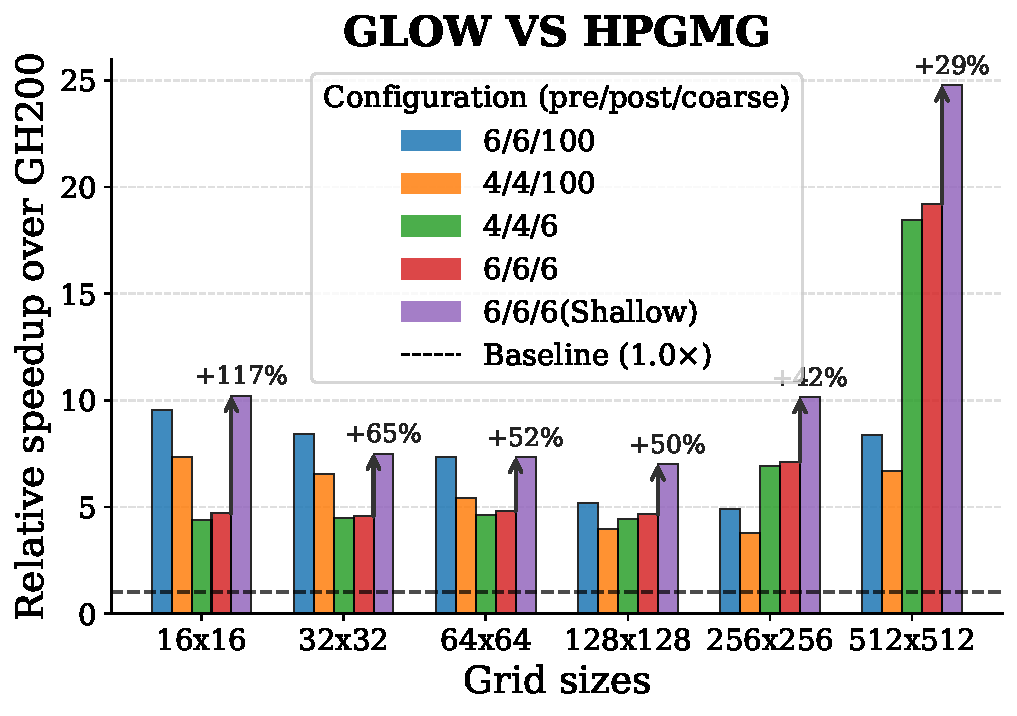
\includegraphics[width=0.95\linewidth]{figures/hpgmg_speedup_barplot.pdf}
                \caption{Speedup comparison between Cerebras CS-3 and NVIDIA GH200 using HPGMG/GLOW across various problem sizes. The bar plot shows relative performance (higher is better). The \% increase indicated on top of 6/6/6(Shallow)(purple) is the relative speedup against the 6/6/6(red). {\color{blue} Timings reflect a single V-cycle only measuring pure operator time, excluding convergence checking cost, on both GPU and WSE.}}
                \label{fig:hpgmg-speedup}
            \end{figure}

            %Several trends explain these results. 
            These performance trends highlight the sensitivity of %multigrid 
            GMG performance on WSE-3 to V-cycle structure. Increasing the number of coarse-level iterations (*/*/6 vs. */*/100) along with depth of the V-cycle %deepens the V-cycle and 
            expands communication distances for both inter-level transfers and intra-level stencil operations. %eventually slowing the solver(We analyze the performance in section \ref{sec:operator-breakdown} in detail). 
            In contrast, our implementation handles finer grids well by scaling the problem over the wafer and exploiting parallelism and stencil locality, with shorter communication distances for halo exchanges and fewer hops to travel for inter-layer communication. A \(6/6/6 (Shallow)\) V-cycle with 7 levels outperforms a \(6/6/6 (Deep)\) V-cycle with 9 levels by almost 45\% on the largest problem size, with the cost of increased iterations to reach convergence.

            As a second observation, speedups grow as problem size scales. GLOW is well suited to finer levels and larger grids, while single-node GPU performance %tend to struggle on 
            worsens on larger problems due to increased data movement through the memory system. %. as the amount of computation on finer grids grows, factors such as data movement costs and memory bandwidth pressure can also become a bottleneck on GPUs at larger grid sizes. 
            %This sentence belongs in the configuration discussion
            %Third, under our current mapping and the 48\,KB per-PE memory limit, we cannot scale beyond a $512\times512$ PE grid. Limiting our experiments for larger problems.

            The configurations with a heavy number of coarse solver iterations (i.e., the blue and orange bars) exhibit a U-shaped trend in Figure~\ref{fig:hpgmg-speedup}, as the cost of the coarse solver dominates for larger problems, pushing the performance to lower levels. Configurations with lighter coarse solver iterations (green and red bars) show a linear increase in performance as the problem scales since very less time is spent on the coarse level. A higher bump on the 512 problem size could also point to how baseline GPUs start struggling with larger grids and not GLOW performing better by 2\(\times\) over previous level.
            %\textcolor{red}{I'm having trouble understanding this.  The U shape for blue and orange shows improvement on both end points although speedup is low.  Maybe be more precise than saying "U-shaped"?}

            %\subsection*{D. Operator Breakdown}
        \subsection{Per-Operator Performance Breakdown}
            We attribute the time spent to
            %We analyze the performance of 
            individual operators in Figure~\ref{fig:per-operation-timing}. %to further explain these results. 
            The plot shows time per operator for one V-cycle on a \(512^3\) problem, summed over each horizontal level (both down and up phases combined). The \(x\)-axis is the multi-grid level from 0 (finest) to 8 (coarsest); the \(y\)-axis is execution time in a log scale (lower is faster). %We explain each line in turn.


            \textbf{Smooth with 7-point (strided) stencil.}
            %\paragraph{Smooth with 7-point (strided) stencil}
            %\textbf{Smoothing (7-point hollow stencil).} 
            %\textcolor{red}{Using "hollow" everywhere is confusing.  It doesn't start out "hollow" -- I prefer the word "strided".  The stride gets larger as the levels increase. I'm commenting out your text, and trying with my own to make this clearer.  Also, it is premature to compare performance to the residual operator that has not been presented.}
            %The smoothing operator, internally implemented using a 7-point hollow-stencil, exhibits behavior similar to that of the residual operator, but with consistently higher cost due to multiple pre and post-smoothing iterations and fixed overheads. As expected, smoothing time initially decreases toward coarser levels because both the number of active PEs and the local data volume are halved at each level. However, unlike conventional weak-scaling behavior reported on CPUs and GPUs[oscar work cite, some GMG CPU/GPU papers] where performance often plateaus/saturates or improves monotonically toward coarser grids, in GLOW we observe a gradual increase in cost beyond a certain level. 
            %The smooth operator is a 7-point stencil.  
            At levels above \(L_1\), a strided stencil refers to skipping PEs in the calculation as a result of the grid coarsening.
            As is typical in GMG, smooth time initially decreases toward coarser levels because both the number of active PEs and the local data volume are halved at each level. However, unlike conventional weak-scaling behavior, %reported on CPUs and GPUs[oscar work cite, some GMG CPU/GPU papers] 
            where performance often plateaus/saturates or improves monotonically toward coarser grids, in GLOW we observe a gradual increase in cost beyond a certain level.

            To better understand this behavior, we microbenchmarked the strided stencil kernel used
            at the heart of the smooth and residual operators, as
            shown in Figure~\ref{fig:spmv-internal}. We measured compute time to calculate the Laplacian across the x-y plane and z-axis. %Whereas 
            Communication time is the time taken to send and receive halo regions to and from neighbors from all 4 directions. Compute time decreases nearly by a factor of two per level before flattening, due to fixed overheads. Communication cost starts lower than compute on finer grids as the stencil halo neighbors are exchanged directly between neighbors, while the data size is largest and has maximal computation.
            %in the best possible locality and both asynchronous, although the data size is larger leading to higher compute costs. 
            The intersection point of these curves reflects the tradeoff between shrinking data volume and increasing communication distance: although each PE processes less data, messages must traverse longer paths as the active region contracts.

            We compare analytical predictions in \ref{tab:model_communication_costs} and Table \ref{tab:comm_model_constant_dl} with these performance measurements.  One can observe the curves with and without forwarding-optimization both show a higher communication cost in the initial finer levels and latency grows as we move towards coarser levels. There is a sweet spot where the communication cost and latency just overlap each other. \textcolor{red}{The following sentence may cause reviewers to say that we should have done this already.  Also, I think it may belong in a subsequent ``Lessons Learned'' section: To further reduce the cost, we believe even more sophisticated techniques to change the routing might be useful, one such is demonstrated by Mathias et al.~\cite{mathias} using control wavelets and runtime coloring reconfiguration.}
            %at the color config and routes level. 
            %I don't know what this means, and I don't think it contributes
            %Another possibility is to teardown the colors before setting each level leading to higher usage of colors which is a limited resource. 
            %We took a simpler approach to short-circuit the queues instead as the cost of resetting the colors and reconfiguring the routes might have been higher summed up over V cycles and iterations.
            %We ran the upstream SDK 7-point stencil (hop-based) and saw similar trends with the turning point shifted toward finer levels.

            \begin{figure}[h!]
                \centering
                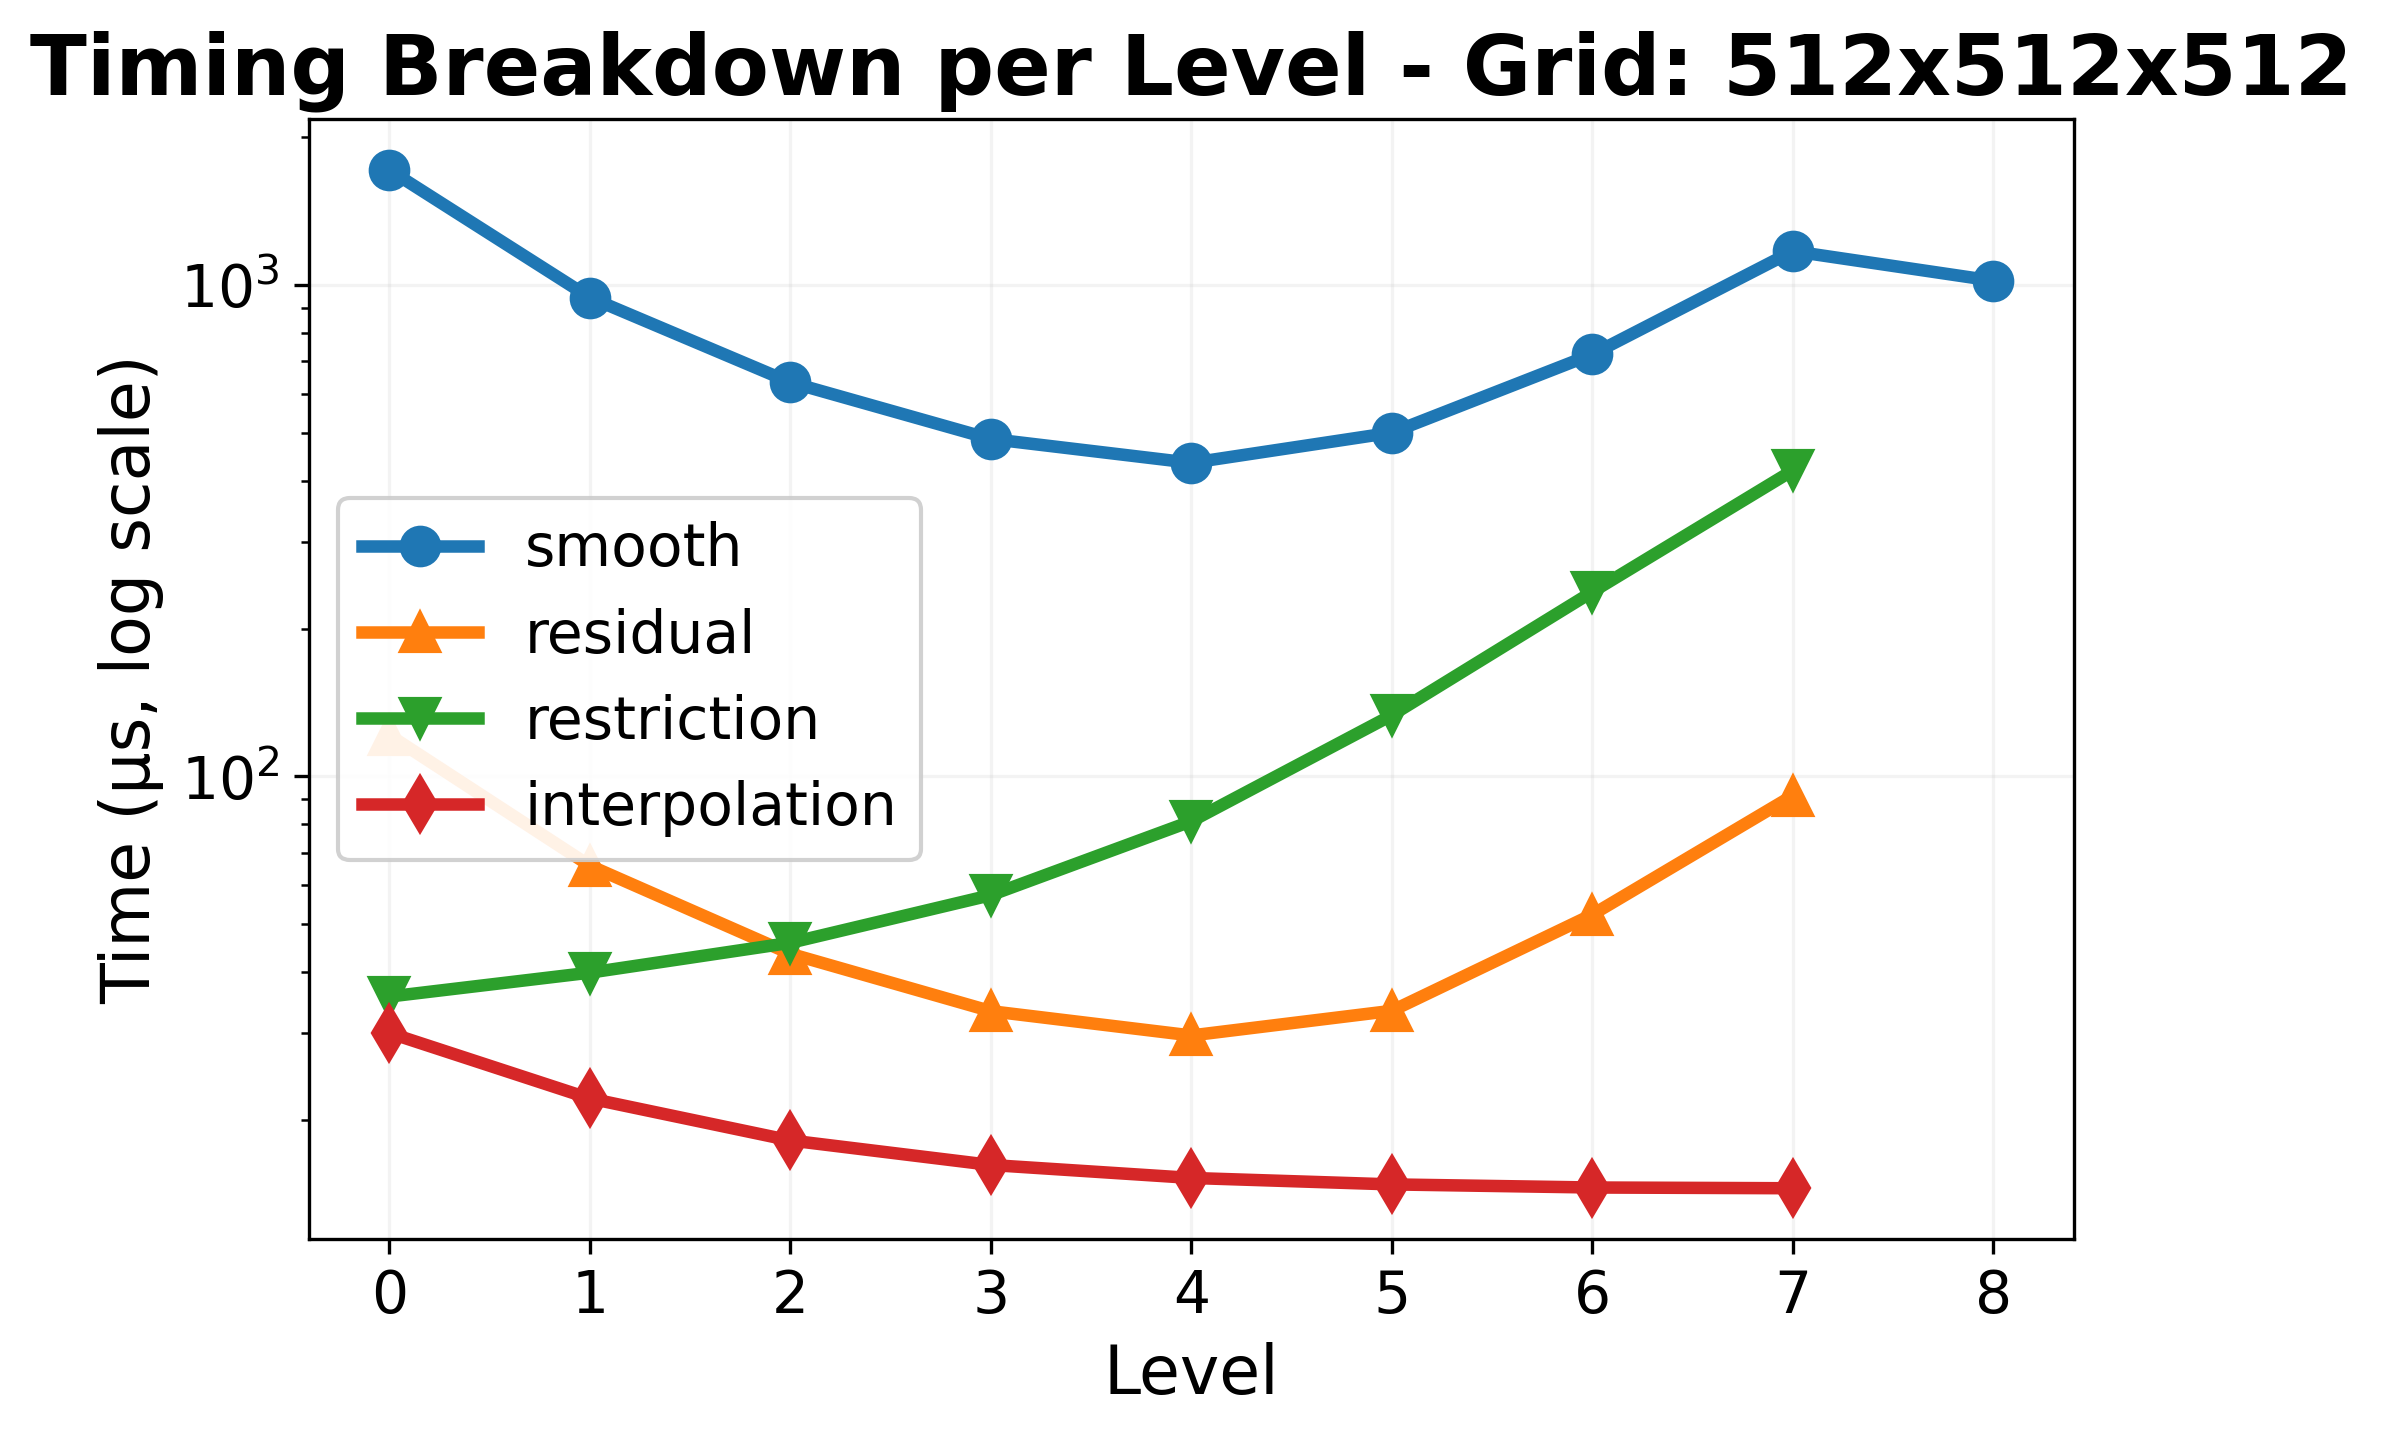
\includegraphics[width=\linewidth]{figures/per_operation_timing_512x512x512.png}
                \caption{Per-operator time per level for one V-cycle on a \(512^3\) problem (GLOW on CS-3). Down and up phases are summed at each level. \(x\)-axis: level 0 (finest) to 8 (coarsest). \(y\)-axis: time (log scale; higher is slower). Config: \(6/6//6\) pre/post/coarse, 9 levels, FP32, 7-point stencil.}
                \label{fig:per-operation-timing}
            \end{figure}

            \textbf{Residual.} The residual operator uses the same 7-point stencil as smoothing and follows a similar performance trend. Differences in absolute time come from the absence of multiple smoothing iterations.

            \textbf{Restriction.} Restriction exhibits increasing cost toward coarser levels. The window-based reduction (Figure~\ref{fig:Spmv_and_restriction}) technique used in our distributed mapping requires contributions from \(N-1\) other PEs within a window, introducing dependence and repeated accesses to local memory via the ramp. As the window size grows relative to the number of active PEs, these dependences dominate execution time. Skipping inactive or out-of-domain PEs during the reduction could potentially reduce this overhead and can be a promising direction for future optimization.

            \textbf{Interpolation:} Interpolation shows the opposite behavior compared to restriction; it is more expensive on finer grids and becomes progressively cheaper toward coarser levels. As microbenchmarked in Figure~\ref{fig:interpolation-internal}, interpolation cost is dominated by sending data compared to computing locally. Although one might expect the cost to increase with distance, instead interpolation benefits from the hardware’s zero-cost multicast capability. Data is broadcast in all four directions simultaneously, allowing row-wise and column-wise transfers to occur in parallel. Unlike restriction, interpolation lacks producer-consumer dependences between PEs, enabling immediate forwarding without intermediate memory accesses.  Consequently, each PE can multicast and advance, thus avoiding the high cost of going down the ramp to memory. As the data volume shrinks at coarser levels, smaller packets are sent over longer distances, but the use of multicast and the avoidance of ramp traffic result in lower overall cost. In Figure~\ref{fig:interpolation-internal}, we see that at each level the window-leader PE (top-left, as shown in Figure~\ref{fig:Spmv_and_restriction}) expands the z dimension, resets the routes, broadcasts data, and eventually when data reaches the destination, calculates the error correction locally using tightly coupled DSD operations. Notice the cost to reset routes is constant mostly.

            % SPMV internal:
            % \begin{figure}[h!]
            %     \centering
            %     
\includegraphics[width=\linewidth]{figures/spmv_internal.png}
            %     \caption{Internal speedup of smooth on Cerebras CS-3 and NVIDIA GH200 using HPGMG and GLOW across various problem sizes. The bar plot shows relative performance (higher is better).}
            %     \label{fig:spmv-internal}
            % \end{figure}
            \begin{figure*}[t]
                \centering
                
\includegraphics[width=\textwidth]{figures/spmv_internal.png}
                \caption{Internal speedup of smooth on Cerebras CS-3 and NVIDIA GH200 using HPGMG and GLOW across various problem sizes. The bar plot shows relative performance (higher is better).}
                \label{fig:spmv-internal}
            \end{figure*}


            % interpolation internal:
            \begin{figure*}[t]
                \centering
                
\includegraphics[width=\linewidth]{figures/interpolation_internal.png}
                \caption{Internal speedup of interpolation on Cerebras CS-3 and NVIDIA GH200 using HPGMG/Glow across various problem sizes. The bar plot shows relative performance (higher is better).}
                \label{fig:interpolation-internal}
            \end{figure*}

            \textbf{Coarse solver.} The coarse solver applies weighted Jacobi relaxation on the coarsest grid. Its cost is very high compared to fine-level operators and grows with the number of coarse iterations. We showed experiments in Figure~\ref{fig:hpgmg-speedup} with varying coarse iterations, significantly impacting overall performance in deep V-cycles.

            % metrics_compare.png
            % \begin{figure*}[t]
            %     \centering
            %     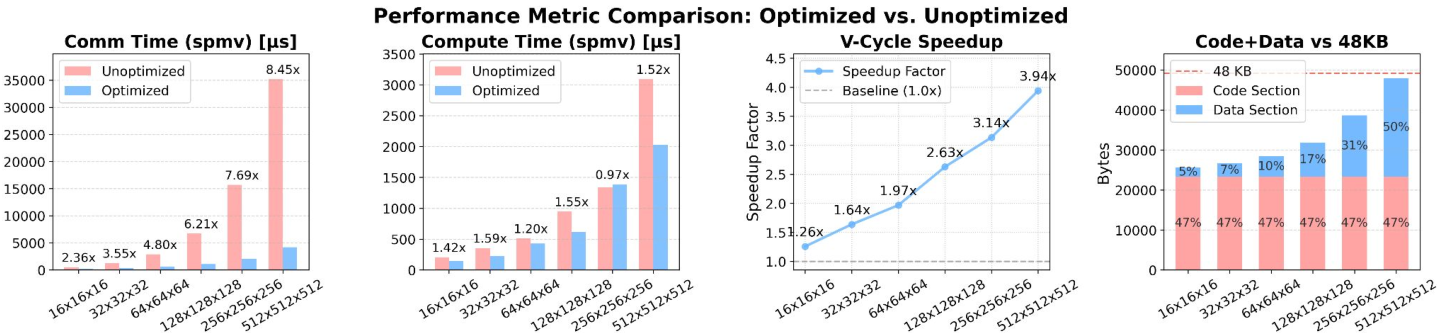
\includegraphics[width=\linewidth]{figures/metrics_comparison_big.pdf}
            %     \caption{Performance of HPGMG/GLOW on Cerebras CS-3 and NVIDIA GH200 using a $512^3$ grid with 9 multigrid levels, up to 100 iterations, a convergence tolerance of $1\times10^{-5}$, $4/4/6$ pre-, post-, and bottom-smoothing steps, float32 precision, Jacobi relaxation $\omega=0.6667$, a 7-point stencil with $\alpha = -6.0$, $\beta = 1.0$, 16 channels, 256 block size, and a $762\times1172$ wafer fabric.}
            %     \label{fig:metrics-compare}
            % \end{figure*}

        \subsection{Forwarding Communication Optimization}
            \label{sec:impact-of-optimizations-and-memory-constraints}
            %\subsection*{E. Impact of optimizations and memory constraints}
            % let's start talking about metrics compare now.
            We further quantify the impact of the forwarding optimization of Section~\ref{sec:forwarding}.
            %our \textcolor{red}{You should have a name for this optimization in the Mapping section, and then you can refer to it by the name.} optimizations 
            in Figure~\ref{fig:metrics-compare}. The forwarding optimization shines as the number of inactive PEs start increasing.  We see almost 8.45\(\times\) speedup over the unoptimized/inactive PE memory accessing implementation. This leads to a 3.94\(\times\) speedup over the whole application shown in the bottom left corner. Compute time reduces since unnecessary computation on inactive PEs is also eliminated.

        \subsection{Memory Constraints: Code vs.\ Data Tradeoff}
            Table~\ref{tab:memory_utilization} quantifies per-PE memory usage across all problem sizes. The code section occupies a fixed ${\sim}$23KB (47\%) of the 48KB SRAM and almost remains constant across problem sizes, this is driven by aggressive function inlining performed by the backend LLVM compiler as well as the inclusion of stencil and collectives library kernels. The data section, which stores solution vectors, residuals, intermediate buffers, and multi-level save arrays, grows from 2.9\% at $4^3$ to 50.7\% at $512^3$, where the PE reaches 98\% capacity. This fixed code footprint combined with geometrically growing per-level data imposes a practical scalability limit: the $512^3$ problem is the largest that fits. Wafer utilization ranges from 0.002\% ($4^3$) to 29.4\% ($512^3$), showing that even our largest problem uses less than a third of the 893,064 available PEs.
            \begin{table}[t]
                \caption{Per-PE memory breakdown and wafer utilization across problem sizes (48KB SRAM per PE, 893,064 total PEs).}
                \label{tab:memory_utilization}
                \centering
                \footnotesize
                \setlength{\tabcolsep}{2pt}
                \begin{tabular}{|r||r|r|r|r|} \hline
                    \textbf{Size} & \textbf{Code} & \textbf{Data} & \textbf{Total} & \textbf{PE Util.} \\ \hline \hline
                    $4^3$   & 23,060 (46.9\%) & 1,440 (2.9\%)   & 49.8\% & 0.002\% \\ \hline
                    $8^3$   & 23,280 (47.4\%) & 1,812 (3.7\%)   & 51.0\% & 0.007\% \\ \hline
                    $16^3$  & 23,280 (47.4\%) & 2,392 (4.9\%)   & 52.2\% & 0.03\%  \\ \hline
                    $32^3$  & 23,272 (47.3\%) & 3,388 (6.9\%)   & 54.2\% & 0.12\%  \\ \hline
                    $64^3$  & 23,276 (47.4\%) & 5,216 (10.6\%)  & 58.0\% & 0.46\%  \\ \hline
                    $128^3$ & 23,276 (47.4\%) & 8,708 (17.7\%)  & 65.1\% & 1.84\%  \\ \hline
                    $256^3$ & 23,272 (47.3\%) & 15,528 (31.6\%) & 78.9\% & 7.34\%  \\ \hline
                    $512^3$ & 23,272 (47.3\%) & 24,908 (50.7\%) & 98.0\% & 29.4\%  \\ \hline
                \end{tabular}
            \end{table}

        {
        \subsection{On V, W and F cycles}
            We chose to investigate only the V-cycle in this paper because it is by far the most common multigrid schedule in practice, and our per-level performance analysis lets the reader translate findings to F-, W-, or $\mu$-cycle variants. From a computational-efficiency standpoint, all parallel architectures favour the V-cycle: it hides coarse-grid latency behind the throughput of fine grids. On the WSE this effect is more pronounced because coarse-grid operations pay a communication cost that grows with level: the active-PE stride doubles per level, the hop distance grows with it, and the low-radix network makes each operation at level $\ell$ increasingly latency-dominated.

            \begin{table}[t]
                \caption{V-cycle vs.\ W-cycle on $256^3$, 8 levels, 6/6/6 (pre/post/coarse) smoothing, $\gamma=2$. Both converge in 10 iterations.}
                \label{tab:vcycle_vs_wcycle}
                \centering
                \footnotesize
                \setlength{\tabcolsep}{3pt}
                \begin{tabular}{|l||r|r|r|} \hline
                    \textbf{Metric} & \textbf{V-cycle} & \textbf{W-cycle} & \textbf{Ratio} \\ \hline \hline
                    Avg cycle time ($\mu$s)       &    483.1 & 15,103.9 & 31.3$\times$ \\ \hline
                    Time to solution ($\mu$s)     &  5,445.6 &151,651.9 & 27.8$\times$ \\ \hline
                    Convergence rate (dec/iter)    &     1.24 &     1.32 &  1.1$\times$ \\ \hline
                \end{tabular}
            \end{table}
            
            As shown in Table~\ref{tab:vcycle_vs_wcycle}, the W-cycle is $31.3\times$ slower per 1 cycle and $27.8\times$ slower to solution as it repeatedly pays coarse-level communication penalty. This confirms that deeper cycle schedules are poorly matched to the strided mapping on WSE also supplemented by our shallow cycle experiments.
        
        }

        {
            \subsection{On Higher-Order Stencils}
            The 7-point constant coefficient stencil is ubiquitous in the computer science performance optimization community. As such, it acts as a necessary first step when analyzing emerging architectures. Sophisticated stencils like 7-point variable coefficient stencils are common in real world applications and 27-point stencils can provide 4th order accuracy, however they might end up with significantly more memory and complicated inter-PE communication patterns. This work uses 7-point constant coefficient stencil which is ubiquitous in computer science performance optimization community. As such, it acts as a necessary first step when analyzing emerging architectures. Given the current state of CSL tooling and library support, a 27-point stencil implementation on WSE is itself a significant contribution as previously highlighted in ~\cite{mathias}.
        }
        
        
        {\color{blue}
        \subsection{Roofline Analysis}
        1. Methodology
        2. Peaks
        3. Insights(1 pe vs N pes)
        compute bound
        discussion on 
            Figure~\ref{fig:roofline} presents a roofline analysis for a $512^3$ problem with 9 levels using 262,144 active PEs. The left panel shows the per-PE (0,0) performance: finer levels (L0, L1) reach 43\% and 18\% of the 1.75 GFLOP/s per-PE peak respectively, operating in the compute-bound region. As levels coarsen, performance drops and shifts toward the memory/fabric-bound region due to growing communication distance and shrinking local computation. The right panel shows the active-PE system view, where the per-level peak scales with the number of active PEs at each level. L0 achieves 43\% of its 458.8 TFLOP/s system peak. The roofline confirms that GLOW is compute-bound at fine levels and transitions to communication-bound at coarse levels, consistent with our per-operator analysis.TODO: Write methodology, and talk about the table<todo add me>

            \begin{figure*}[t]
                \centering
                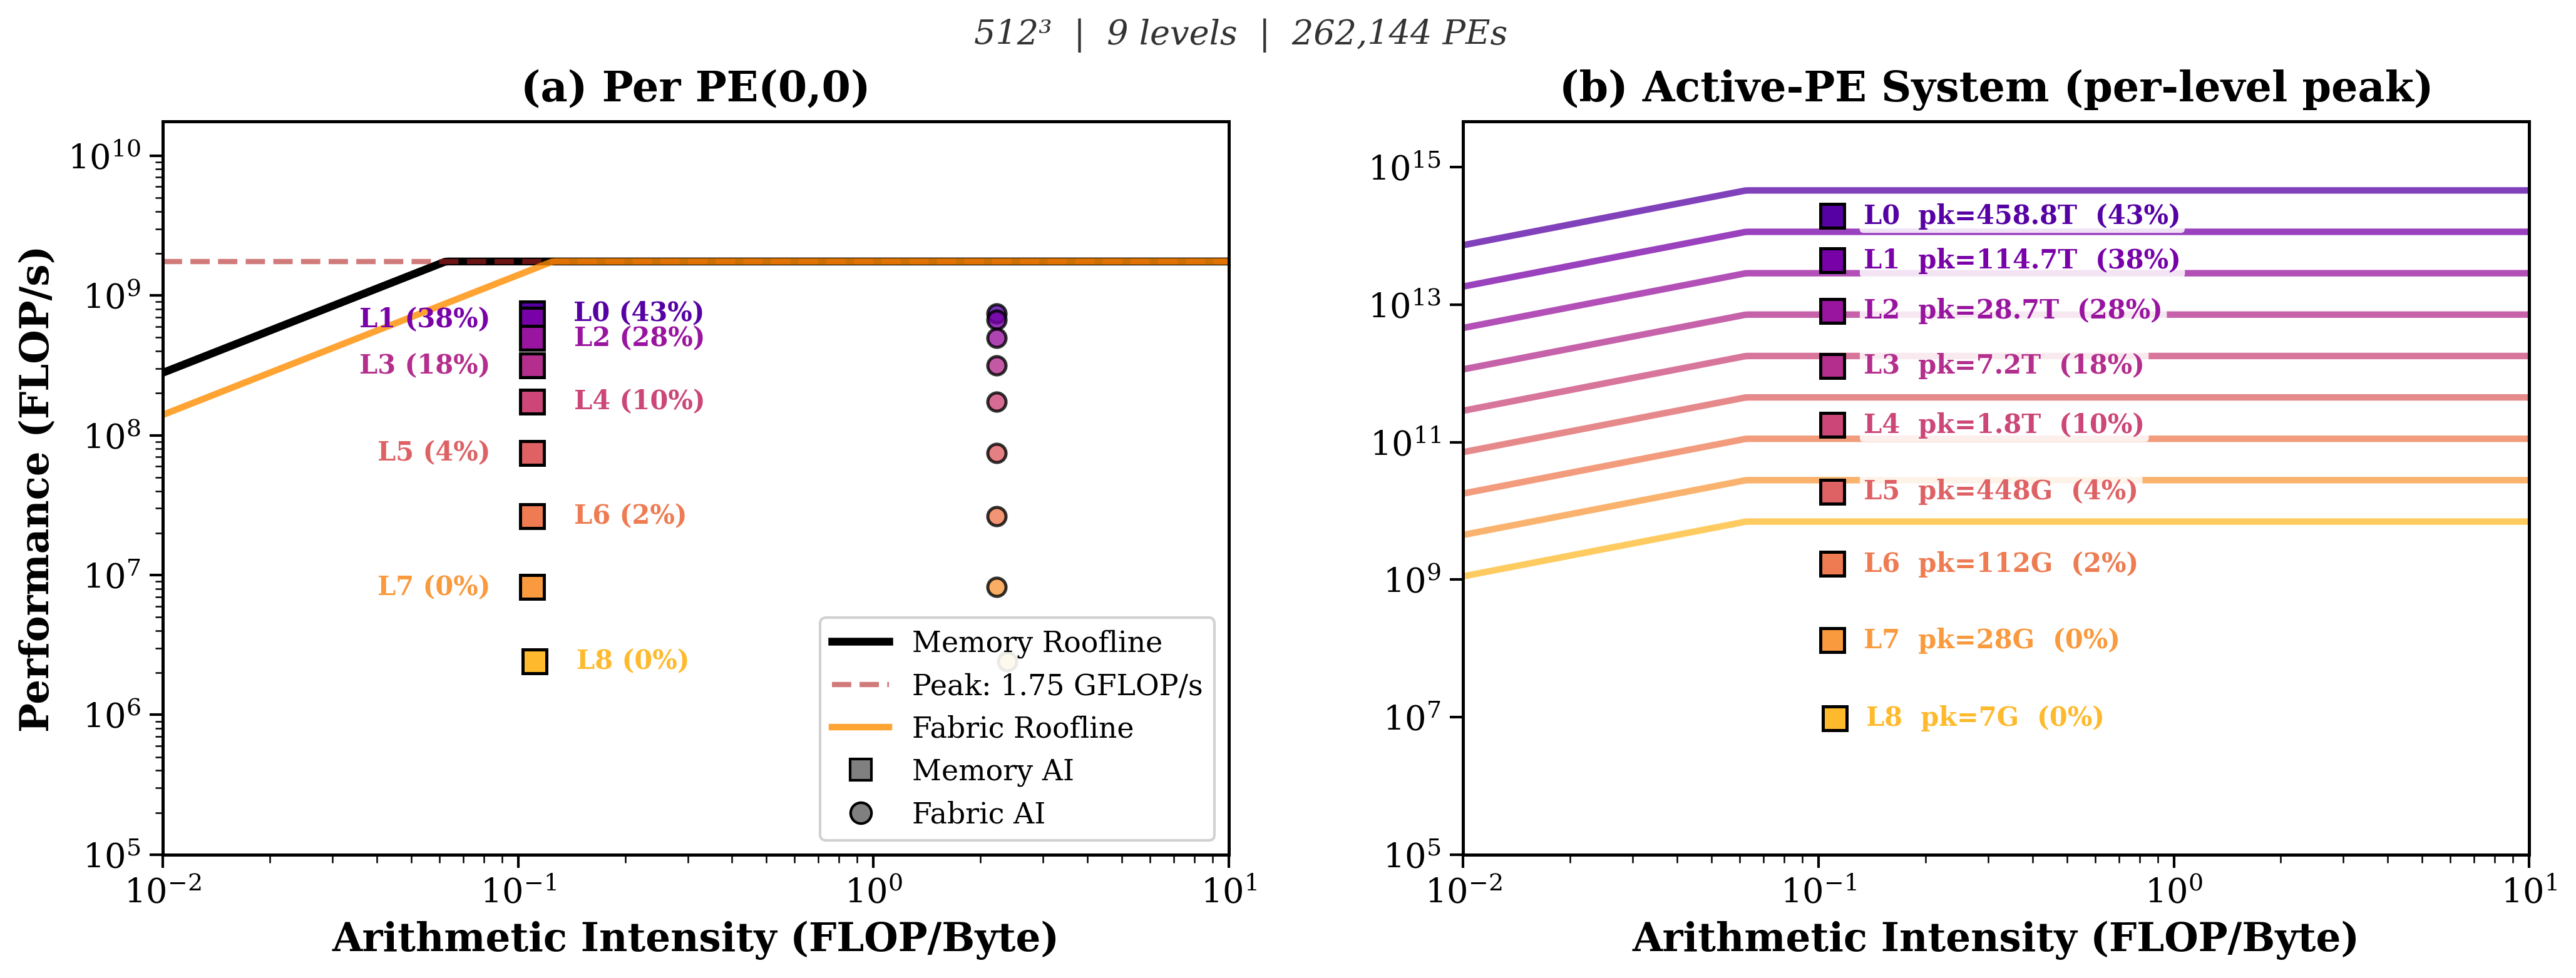
\includegraphics[width=\textwidth]{figures/roofline_plot.png}
                \caption{Roofline analysis for $512^3$ with 9 levels. Left: per-PE performance vs.\ arithmetic intensity. Right: system-level performance scaled by active PEs per level. Dashed line: 1.75 GFLOP/s per-PE peak.}
                \label{fig:roofline}
            \end{figure*}

            \begin{table}[t]
                \caption{Per-PE operation breakdown for a $512^3$ V-cycle. Count is the number of times the operation executes. FLOPs is the arithmetic work (FMAC counts 2 FLOPs per operation; FMOV variants contribute 0). Mem(B) is total SRAM traffic: $(loads + stores) \times 4$ bytes. Fab(B) is fabric traffic from halo exchange; only FMOV32 touches the fabric. Mem AI = Total FLOPs / Mem(B); Fab AI = Total FLOPs / Fab(B).}
                \label{tab:roofline_ops}
                \centering
                \footnotesize
                \setlength{\tabcolsep}{2pt}

                \vspace{2pt}
                \textbf{Level 0 ($512^2$ PEs)}
                \vspace{1pt}

                \begin{tabular}{|l||r|r|r|r|} \hline
                    \textbf{Op} & \textbf{Count} & \textbf{FLOPs} & \textbf{Mem(B)} & \textbf{Fab(B)} \\ \hline \hline
                    FSUB      &   79,872 &   79,872 &    958,464 &       0 \\ \hline
                    FMAC      &  632,832 & 1,265,664& 10,125,312 &       0 \\ \hline
                    FMUL      &    3,072 &    3,072 &     36,864 &       0 \\ \hline
                    FADD      &   21,504 &   21,504 &    258,048 &       0 \\ \hline
                    FNEG      &  159,744 &  159,744 &  1,277,952 &       0 \\ \hline
                    FMOV\_MEM &   36,352 &        0 &    290,816 &       0 \\ \hline
                    FMOV\_ZERO&   92,160 &        0 &    368,640 &       0 \\ \hline
                    FMOV32    &  172,033 &        0 &    688,132 & 688,132 \\ \hline \hline
                    \textbf{Total} & & \textbf{1,529,856} & \textbf{14,004,228} & \textbf{688,132} \\ \hline \hline
                    \multicolumn{3}{|l||}{\textbf{Mem AI}: 0.109} & \multicolumn{2}{l|}{\textbf{Fab AI}: 2.223} \\ \hline
                \end{tabular}

                \vspace{4pt}
                \textbf{Level 7 ($4^2$ PEs)}
                \vspace{1pt}

                \begin{tabular}{|l||r|r|r|r|} \hline
                    \textbf{Op} & \textbf{Count} & \textbf{FLOPs} & \textbf{Mem(B)} & \textbf{Fab(B)} \\ \hline \hline
                    FSUB      &      624 &      624 &      7,488 &       0 \\ \hline
                    FMAC      &    4,944 &    9,888 &     79,104 &       0 \\ \hline
                    FMUL      &       24 &       24 &        288 &       0 \\ \hline
                    FADD      &      168 &      168 &      2,016 &       0 \\ \hline
                    FNEG      &    1,248 &    1,248 &      9,984 &       0 \\ \hline
                    FMOV\_MEM &      240 &        0 &      1,920 &       0 \\ \hline
                    FMOV\_ZERO&      768 &        0 &      3,072 &       0 \\ \hline
                    FMOV32    &    1,344 &        0 &      5,376 &   5,376 \\ \hline \hline
                    \textbf{Total} & & \textbf{11,952} & \textbf{109,248} & \textbf{5,376} \\ \hline \hline
                    \multicolumn{3}{|l||}{\textbf{Mem AI}: 0.109} & \multicolumn{2}{l|}{\textbf{Fab AI}: 2.223} \\ \hline
                \end{tabular}
            \end{table}

            Table~\ref{tab:roofline_ops} breaks down the per-PE operations at the finest (L0) and a coarse level (L7). FMAC (multiply-accumulate from the stencil) dominates the FLOPs, while FMOV32 is the only operation that touches the fabric (halo exchange). The arithmetic intensity is constant across levels (0.109 FLOP/Byte for memory, 2.223 FLOP/Byte for fabric), but absolute work shrinks by $128\times$ from L0 to L7. Coarse levels have too little computation to amortize fixed communication overheads (router latency, growing hop distance), explaining the transition from compute-bound to communication-bound in Figure~\ref{fig:roofline}.
        }

    \section{Lessons Learned and Next Steps}
        {\color{blue}
        \paragraph{Mapping layered algorithms to spatial architectures.(moved from top)}
        Mapping a multi-level algorithm like GMG onto a spatial dataflow architecture requires balancing several competing concerns: memory footprint per PE, communication distance between levels, packing/repacking cost, stencil locality, chip utilization, and routing/coloring complexity. No single layout strategy dominates across all of these dimensions; the strided distributed mapping we chose prioritizes stencil parallelism and avoids bulk inter-level data movement, but at the cost of growing communication distance at coarser levels.}

        \textcolor{red}{Grabbed from above:
        SOME INTRO PARAGRAPH...
        \paragraph{Further improvements to forwarding optimization.}
        To further reduce the cost, we believe even more
        sophisticated techniques to change the routing might be useful, one
        such is demonstrated by Mathias et al.~\cite{mathias} using control wavelets and runtime coloring reconfiguration.
        \paragraph{Addressing constrained memory size.}
        Revisit 512-cubed...Future approaches may benefit from hybrid mapping strategies that decouple computation and storage, such as assigning subsets of PEs primarily as memory resources while others focus on computation, or employing more dynamic coloring and routing schemes to reduce code replication and improve memory utilization across levels.}

        1. Various mapping (???), localized based on application as much as possible, memory constraints.
        2. Conventional distributed mappings,
        3. Pipeline for this application doesn't make sense, partition problems, distance
        4. Programming model(async and hangs), colorings(design sophscticated patterns)
        5. Mppaing, memory, distance of communication, convergence(HPC low radix machines for larger distances and cerebras needs to think about it), uniform communication patterns.
        6. Poeple should not have to go to 27pt because of what oscar explained me, write it. They choose 27 pt because say 7pt was memory bound and using 27 pt the performance at least moves up, now given that GLOW is alredy compute bound we can't get speedups using 27pt as we are already there, one benefit is of accuracy using 27pt. there can be other implications, say 27 will be less power hungry.


    \section{Related Work}
        %\paragraph{Stencils and GMG}
        Historically, operations on large structured grids could easily be bound by capacity misses in cache, leading to a variety of studies on blocking and tiling optimizations to improve cache reuse on CPUs%[6, 8, 15, 19, 20, 27, 28].
        %(an incomplete list might include
        ~\cite{Nguyen:2010:BOS:1884643.1884658,Zhou:2012,Yount:2016:YSK:3019129.3019133,Unat2016,Devito}. These techniques for multigrid have been successfully applied to finite-difference and finite-volume discretizations on shared-memory and distributed-memory systems.
        As new supercomputer architectures evolve with higher peak multi-node performance, the growing gap between DRAM bandwidth and floating point operations (FLOPs) has focused research on increasing performance through data locality, particularly for bandwidth-bound computations.

        Other efforts have introduced MG frameworks that could
        efficiently exploit resources on GPU architectures. Examples
        of recent multiphysics applications, where multigrid solvers
        are key for elliptic equations, on structured or unstructured
        grids include~\cite{Amrex,Anderson,Grete,mali}. Many of these efforts have been
        focused on GPU acceleration and, to some extent performance
        portability, since the focus is on different supercomputers with
        different GPU vendors. However, because of the complexity
        of multigrid solvers, it is an ongoing challenge to do detailed
        performance analysis and explore optimization techniques
        that exploit increasing GPU parallelism, GPU memory, and
        network bandwidth.



        %\paragraph{Stencils and Geometric Multigrid}
        %~\cite{Nguyen:2010:BOS:1884643.1884658,Zhou:2012,Yount:2016:YSK:3019129.3019133,Unat2016,Devito}. 

\begin{comment}
            \paragraph{Wafer-Scale Computing for Scientific Applications}
            Several studies have ported scientific applications to wafer-scale architectures.
            (add links)  Purely stencil. Larger applications. Programming stacks.
            \begin{itemize}
            \item High-order stencil computations achieving near-perfect weak scaling~\cite{Sai,sai2}.
            \item Matrix-free finite-volume solvers for subsurface flow.
            \item Molecular dynamics simulations breaking timescale barriers.
            \item Monte Carlo particle transport kernels with over 100× GPU speedup.
            \item Communication collectives (Reduce/AllReduce) optimized for wafer-scale fabrics.
            \end{itemize}
            No published work has yet demonstrated GMG on Cerebras, making this study the first exploration.
\end{comment}
        A growing body of work has demonstrated the effectiveness of wafer-scale systems for scientific computing. Early studies showed near-ideal weak scaling for high-order stencil computations and structured finite-difference operators on the WSE~\cite{scalable_25pt_stencil,Rocki,mathias,Sai,sai2}. Subsequent work extended these ideas to matrix-free finite-volume solvers for subsurface flow and seismic applications, highlighting the advantages of spatial data placement and explicit communication control~\cite{sai_fv_arxiv,Ltaief}. Larger application studies include molecular dynamics simulations that overcome traditional timescale barriers~\cite{perez_md_sc24,perez-journal} and Monte Carlo particle transport kernels achieving substantial speedups over GPU-based implementations~\cite{Tramm24,Yoshii26}. Communication-intensive primitives such as reductions and all-reductions have also been studied in isolation, with near-optimal collective implementations demonstrated on wafer-scale fabrics~\cite{luczynski_reduce}.

        In parallel, several efforts have focused on improving programmability and compiler support for wafer-scale systems. These include DSL-based approaches for stencil computation~\cite{brown}, automated code generation for high-order stencils~\cite{sai_codegen_sc24}, and MLIR-based lowering pipelines targeting spatial dataflow architectures~\cite{stawinoga_mlir_stencils_wse}.
        SPADA~\cite{spada} is a programming language targeting spatial architectures that provides precise control over data placement, dataflow patterns, and asynchronous operations while abstracting architecture-specific low-level details. Various literature on analytically modeling and spatial algorithmic primitives have been explored as well~\cite{gianinazzi_spatialcomputer, gianinazzi2025energy, baumann2024low, luczynski_reduce}.
        While these works significantly advance kernel-level performance and developer productivity, they primarily target single-level stencil operators or application-specific kernels.%[spada is missing?]

        To the best of our knowledge, no prior work has demonstrated a complete geometric multigrid solver mapped onto a wafer-scale architecture. GMG introduces additional challenges beyond single-level stencils, including multi-level data grids, coarse-grid solvers, and level-dependent communication patterns. This work represents the first end-to-end exploration of mapping a full GMG algorithm onto the Cerebras WSE-3 system, bridging the gap between prior stencil-centric studies and full multi-level scientific solvers.


\begin{comment}
            I am commenting this out -- it breaks the flow, and it will be more work to do this well.
            \textcolor{blue}{
            Question: Is it worth to point what's happening in AI world for mapping layers on GPUs/WSE3?  This can connect AI layered mappings on Multigrid and show connection. Discard if not.
            }
            %* CNN mapping can be related work/any layered mapping application/algorithm.
            * CNN mapping can be related work/any layered mapping application/algorithm.
            * Distributed training of AI models and types of parallelism used - data parallel, model parallel, pipeline parallel, etc.
            https://towardsdatascience.com/distributed-parallel-training-data-parallelism-and-model-parallelism-ec2d234e3214/
\end{comment}

\begin{comment}
            \section{Lessons Learned}
            \begin{itemize}
            \item Stencil-style, matrix-free kernels align best with CS-3; use them when structure allows.
            \item AMG coarse operators generally require explicit sparse storage; use CSR/block-CSR within a PE and communicate only among nonzero-owning PEs.
            \item Colors and custom routing schedules are indispensable to avoid contention and ensure determinism.
            \item Developers must embrace matrix-free, fused-kernel approaches rather than porting sparse matrix libraries directly.
            \item AMG represents the next step toward evaluating the architecture’s ability to handle irregular, graph-like scientific computations.
            \end{itemize}
            \textcolor{blue}{
            \textbf{Lessons Learned:(dump, maybe not suitable here}
            * Hardware fast, hard to program.
            * Programming async and dataflow a new way of thinking compared to GPU(threadbased)
            * Using AI for non-AI
            * Tiled baseds hardwares and tiled based IR/Languges.
            * Not right hardware for some type of applications.
            * Memory is issue, need a shared + Distributed way to program this machine.
            * Tooling debugger, profilers essential to have.
            * shallower V-cycles are better matched to the wafer-scale architecture
            \subsection*{Key Discussion/Take aways from results:}
            \begin{itemize}
            \item We observe the GLOW is compute bound on finer levels and communication bound on coarser levels.
            \item We observe having deep V cycles versus shallower V cycles yields significantly higher speedups with the cost of increased iterations to reach convergence.
            \item We think this application might not be a right fit for this architecture, we believe having a scaled out parallelism benefits from this machine rather than a distance dominating.
            \item We found having locality of data across PEs is the equivalent of data movement cost or cache equivalent costs in GPUs/CPUs. - Rewrite this
            \end{itemize}

            }
\end{comment}
    \section{Conclusion}
        We presented a mapping of GMG to WSE-3, achieving up to a \(25\times\) speedup over a single node NVIDIA H200 GPU.  As this is, to our knowledge, the first mapping of GMG to WSE-3, this work exposes the challenges of achieving efficiency for layered algorithms, especially when memory size is so constrained. As a result of this work, we make a number of observations regarding mapping multigrid algorithms to tiled architectures.  First, the compute time dominates for the fine grids, but communication time dominates and increases execution time for coarser grids due to the strided communication.  Therefore, shallow versus deep V-cycles or W-cycles are better suited for this architecture. The communication pattern required to skip over inactive PEs was optimized with a forwarding optimization that lead to significant speedups for coarse grids.
        In spite of these challenges, deterministic, high-bandwidth memory access times and local network bandwidth lead to speedups over a single GPU.


        %that balances matrix-free efficiency with matrix-based generality. %Conceptual tables and figures clarify the programming model and architectural trade-offs. Future work will add empirical results, refine placement/routing for coarse levels, and explore portable abstractions for dataflow multigrid. AMG poses both opportunities and challenges on wafer-scale architectures. By reinterpreting its sparse, memory-bound kernels as streaming dataflow, we can leverage the WSE’s massive bandwidth and low-latency interconnect. Our analysis shows potential for compute-bound SpMV, efficient fine-level scaling, and bottlenecks at coarse levels. Future work will complete performance evaluation, explore adaptive coarsening layouts, and develop portable abstractions for AMG on dataflow hardware.
\begin{comment}
            \item \textbf{Sparsity representation:} AMG is well suited for unstructured problems,
            where PDE discretizations\cite{b12} generate sparse matrices with highly irregular patterns.
            Mapping such irregular sparsity efficiently onto WSE is non-trivial.

            \item \textbf{Communication bottlenecks:} Although the hardware fabric is low-latency,
            AMG relies heavily on SpMV kernels. These can become communication-bound as both the
            problem size and the PE grid size scale up, leading to potential bottlenecks across the wafer.

            \item \textbf{Routing limitations:} On WSE, communication links must pass through intermediate PEs.
            Skipping over PEs that correspond to zero entries (as might be desirable in sparse operations)
            is not feasible given hardware constraints.

            \item \textbf{Sparse matrix mapping challenge:} The problem essentially reduces to mapping a
            sparse matrix across the wafer. While a local PE submatrix could use formats like BlockCSR
            to reduce intra-PE operations, the irregular nature of input sparsity remains a major obstacle.

            \item \textbf{Irregular access and communication:} AMG is a general solver, but its irregular
            communication and data access patterns conflict with the mesh-based organization of WSE.

            \item \textbf{Open research direction:} Mapping irregular sparsity efficiently on WSE may
            require revisiting older sparse data structures (previously deemed obsolete) or developing
            entirely new ones tailored to large-scale, distributed wafer architectures.
            \end{itemize}

            \textbf{Matrix way partitioning strategy}
            Instead of giving a processor a full row or column (which would require a lot of memory), checkerboard partitioning divides the sparse matrix into a grid of submatrices. A processor at location (i,j) in your PE grid is responsible for the submatrix Aij and the corresponding parts of the input vector xj and output vector yi.
            Load Balancing: A simple uniform checkerboard might not work well for an irregular sparse matrix. To ensure even work distribution, you should use graph partitioning algorithms (like those from the Mondriaan or ParMETIS libraries) to cut the matrix into blocks that have roughly the same number of non-zero elements.
            Memory Efficiency: By distributing the matrix non-zeros and vector elements across a million PEs, the memory requirement per PE becomes minimal. This is the only way to handle a large matrix on hardware with very little memory per processing unit.
            2. Communication Strategy
            The SpMV operation on a 2D grid involves two communication phases:
            Column-wise Communication (Gather): Each processor (i,j) needs its part of the input vector xj. This means that all PEs in a given column of the processor grid must receive the same portion of the input vector. A broadcast or a collective gather operation along the processor columns is ideal for this. The PE that ``owns'' the j-th part of the vector x sends it to all PEs in its column.
            Row-wise Communication (Accumulation): After each PE computes its partial result (Aijxj), these partial results must be summed up to form the final output vector y. This requires each PE (i,j) to send its partial result to all other PEs in its processor row. The final result yi is the sum of all partial results from the PEs in row i of the processor grid. This is typically done using a reduction or all-reduce operation along the processor rows.
\end{comment}


%\section*{References}
\bibliographystyle{IEEEtran}
\bibliography{references}
\vspace{12pt}
\end{document}
